%%%%%%%%%%%%%%%%%%%%%%%%%%%%%%%%%%%%%%%%%
% Author: Lanqin Yuan
% fyempathy@gmail.com
% License:
% CC BY-NC-SA 3.0 (http://creativecommons.org/licenses/by-nc-sa/3.0/)
%
%%%%%%%%%%%%%%%%%%%%%%%%%%%%%%%%%%%%%%%%%

%----------------------------------------------------------------------------------------
%	PACKAGES AND DOCUMENT CONFIGURATIONS
%----------------------------------------------------------------------------------------

%\documentclass{article}
\documentclass[a4paper, 11pt, oneside]{Thesis} % use thesis latex class

%\usepackage[margin=2cm]{geometry} % Set margins to whatever
\usepackage{graphicx} % Required for the inclusion of images
\usepackage{natbib} % Required to change bibliography style to APA
\usepackage{amsmath} % Required for some math elements 
\usepackage{float}
\usepackage{algorithm}% http://ctan.org/pkg/algorithms
\usepackage{algpseudocode}% http://ctan.org/pkg/algorithmicx
% ---
% makes sure figures doesnt screw up sections and subsections
\usepackage{placeins}
\let\Oldsection\section
\renewcommand{\section}{\FloatBarrier\Oldsection}
\let\Oldsubsection\subsection
\renewcommand{\subsection}{\FloatBarrier\Oldsubsection}
\let\Oldsubsubsection\subsubsection
\renewcommand{\subsubsection}{\FloatBarrier\Oldsubsubsection}
% ---

%\setlength\parindent{0pt} % Removes all indentation from paragraphs

%\renewcommand{\labelenumi}{\alph{enumi}.} % Make numbering in the enumerate environment by letter rather than number (e.g. section 6)

%\usepackage{times} % Uncomment to use the Times New Roman font

%----------------------------------------------------------------------------------------
%	DOCUMENT INFORMATION
%----------------------------------------------------------------------------------------

\begin{document}
% Insert Title Page
\begin{titlepage}

\newcommand{\HRule}{\rule{\linewidth}{0.5mm}} % Defines a new command for the horizontal lines, change thickness here

\center % Center everything on the page
 
%----------------------------------------------------------------------------------------
%	HEADING SECTIONS
%----------------------------------------------------------------------------------------

\textsc{\Large University of Waikato}\\[5cm] % Name of your university/college

%----------------------------------------------------------------------------------------
%	TITLE SECTION
%----------------------------------------------------------------------------------------

\HRule \\[0.4cm]
{ \huge \bfseries Exploration of Feature Selection Techniques for Data Stream Mining}\\[0.2cm] % Title of your document
\HRule \\[0.4cm]
 
\textsc{\LARGE COMP 520}\\[0.1cm] % Major heading such as course name
\textsc{\large Project report}\\[0.4cm] % Minor heading such as course title
%----------------------------------------------------------------------------------------
%	AUTHOR SECTION
%----------------------------------------------------------------------------------------

\begin{minipage}{0.4\textwidth}
\begin{tabular}{l l l}
\large
\emph{Author:} & & Lanqin \textsc{Yuan} \\
\emph{Supervisor:} & & Bernhard \textsc{Pfahringer}

\end{tabular}
\end{minipage} \\[0.5cm]
%----------------------------------------------------------------------------------------
%	DATE SECTION
%----------------------------------------------------------------------------------------

{\today} % Date, change the \today to a set date if you want to be precise


\vfill % Fill the rest of the page with whitespace


%----------------------------------------------------------------------------------------
%	LOGO SECTION 
%----------------------------------------------------------------------------------------
\begin{center}


\includegraphics[width=0.35\linewidth]{waikatoLogoBig}
%
\includegraphics{waikatoLogoBig} % Include a department/university logo - this will require the graphicx package

This report is in partial fulfilment of the requirements for the degree of
Bachelor of Computing and Mathematical Sciences with Honours
(BCMS(Hons)) at the University of Waikato.

\end{center}


%----------------------------------------------------------------------------------------
%	COPYRIGHT SECTION
%----------------------------------------------------------------------------------------
% TODO Insert copyright stuff here


 
%----------------------------------------------------------------------------------------

\end{titlepage}
\clearpage

\cleardoublepage

\pagestyle{empty}  % No headers or footers for the following pages

\null\vfill
% Now comes the "Funny Quote", written in italics
\textit{``Nature never deceives us; it is we who deceive ourselves.''}

% who said the quote
\begin{flushright}
Jean-Jacques Rousseau
\end{flushright}

\vfill\vfill\vfill\vfill\vfill\vfill\null
\clearpage  % Funny Quote page ended, start a new page



\setstretch{1.3}  % Reset the line-spacing to 1.3 for body text (if it has changed)

% The Acknowledgements page, for thanking everyone
\acknowledgements{
%\addtocontents{toc}{\vspace{1em}}  % Add a gap in the Contents, for aesthetics

I would like to express my gratitude to all my friends for their support. I give a special thanks Jeff Mo for his help, advice, and feedback, always being someone of whom I can bounce ideas off of. I also give special thanks to Antonia McGhie for giving many hours of her free time to help me with proofreading, and Bob Lu for also spending his personal time to help with proofreading.

A special mention and gratitude to my mum for providing me with copious amounts of food.

I would also like to acknowledge and thank Jean-Paul Barddal, for providing me with implementations of PiD and DFW.

Last but not least, many thanks go to my supervisor Bernhard for his help, guidance, and encouragement throughout the project.

}
\clearpage  % End of the Acknowledgements

% FRONTMATTER
\pagenumbering{roman} % Begin Roman style (i, ii, iii, iv...) page numbering

% insert a table of contents
\tableofcontents
\listoffigures
 
\listoftables
\clearpage


\addtotoc{Abstract}
\begin{abstract}
%\addtocontents{toc}{\vspace{1em}}  % Add a gap in the Contents, for aesthetics
Feature selection has been studied and shown to improve performance in standard batch data mining but is mostly unexplored in data stream mining. The flowing and potentially infinite nature of data streams demand that algorithms in a stream setting be efficient, constrained in memory usage, and incremental. Algorithms must also be able to cope with changes in the stream's distributions which can occur at any time. Our project explores subsetting as a method of feature selection in a stream setting and investigates its effectiveness in addressing the aforementioned problems. We propose a new method of embedded feature subset selection specialised for kNN classification in a stream setting based called Iterative Subset Selection (ISS) which splits the feature selection into two stages, first ranking the features, then iteratively selecting features from the ranking. We implement and test the method against a variety of datasets and from our results we conclude that the proposed feature selection method does improve overall classifier performance.
%\addcontentsline{toc}{chapter}{Abstract} % add abstract to

\end{abstract}

\clearpage % next page


% MAINMATTER
\pagenumbering{arabic}
\pagestyle{fancy}
%----------------------------------------------------------------------------------------
%	SECTION 1
%----------------------------------------------------------------------------------------
\chapter{Introduction}
\label{chapter:Introduction}

The selection of relevant features to be considered by the training algorithm in a batch data mining setting has been shown to be beneficial to prediction performance as well as improving computation time and memory usage \citep{Hall98correlation-basedfeature}. Considering too many features during training can result in over-fitting which can lead to poor classification prediction rates. Features which are irrelevant to the task at hand also take up valuable memory and are a burden to computation time while not actually improving, or in some cases worsening classification prediction performance by causing the classifier to overfit.

As data stream mining is a relatively new area in the field of data mining and machine learning, feature selection in a stream setting has so far been a mostly ignored area of study. Adapting batch feature selection algorithms to a stream setting is not straightforward due to the constraints of the stream setting previously mentioned and as a result feature selection algorithms specialised for data stream mining are far and few.

For our project, we propose and explore a new technique for feature selection specialised for a stream setting. We implement this method and test its effect on classifier accuracy, computation time, and memory usage in a variety of different stream settings.

%----------------------------------------------------------------------------------------
%	SECTION 2
%----------------------------------------------------------------------------------------
\chapter{Related Work}
\label{chapter:RelatedWork}
\section{Feature selection for batch bata}

Feature selection as a means of preprocessing data for data mining to improve performance has been studied previously. In general, feature selection techniques can be broadly split into three separate categories: filter methods, wrapper methods, and embedded methods \citep{Guyon:2003:IVF:944919.944968}.

\subsection{Filter methods}
Filter methods evaluate the data individually and independently from a classifier. Methods tend to have low computational complexity which makes them fast and also inexpensive memory wise. Independence from the classifier makes filter methods generally resilient to overfitting but means that the features selected are not optimised for the classifier. Also as the features are evaluated independently from each other, filter methods tend to not consider relationships which exist between the features themselves.

\subsection{Wrapper methods}
Wrapper methods wrap around specific classifiers and utilise the classifier as a black box to select a subset of features based on the subset's usefulness to the specific classifier. Relationships between features are considered and the classifier is also considered in the feature selection process; however wrapper methods tend to be more expensive in terms of computation time and memory usage compared to the simpler filter methods and also tend to be more prone to overfitting.

\subsection{Embedded methods}
Embedded methods are like wrapper methods in that they select a subset of features; however unlike wrapper methods, embedded methods are integrated into the construction or learning of the classifier rather than viewing the classifier as a black box. Embedded methods tend to perform with less computational cost than wrapper methods while still considering subsets of features. The trade-off of embedded methods is that methods tend to need to specialise for the classifier and are not modular with other classifiers.

\subsubsection{ESFS}
The starting point of our new feature selection method was an existing batch feature selection method called ESFS (Embedded Sequential Forward Selection) \citep{ESFS}. ESFS itself is based upon the simple greedy, bottom up wrapper method of SFS (Sequential Forward Selection).

The ESFS method creates an initial ranking of features based on belief mass from Dempster-Shafer theory \citep{dempster1967} and utilises this ranking to cull features below a threshold from the next stage of feature selection. ESFS uses a heuristic search to explore the subset space; starting with individual features as subsets, the method searches through the different combinations of subsets. Subsets are evaluated and culled based on their performance and computational burden according to a user set threshold and re-added into the search as features. This is repeated until all sizes of subsets are covered and a final subset is selected when no more new subsets above the threshold can be created.

As ESFS is proposed for standard batch learning, issues exist which prevents it from working well in a stream setting. Searching for all combinations of subsets of features is a $\mathcal{O}(\min \left(n^k, n^{n-k}\right))$ polynomial problem and despite ESFS's heuristic approach to the computation of subsets, it is still expensive in regards to an algorithm for a stream setting. Computing the belief mass to rank features is also computationally expensive and more importantly requires a distinctly separate training and test set, which is not straightforwardly achievable in an incremental stream setting due to examples potentially arriving unevenly and the possibility of change within the stream.

\section{Feature selection for stream mining}
Recent studies have shown promising improvements which can be obtained by applying feature selection to data streams, especially in terms of addressing feature drift \citep{Barddal2016}. Feature drift is defined as when a feature or subset of features emerges or ceases to be relevant to the classification problem in the stream. Feature drift has mostly been an understudied type of drift in data stream mining and has been shown to negatively affect performance in classifiers when they occur \citep{Barddal2015}.

\section{kNN in stream mining}
For the purposes of our project, we chose to focus on kNN as our classifier to limit the scope of the project. Research has shown kNN to be a robust and high performing method for a wide range of data streams \citep{Read2012}. A beneficial characteristic of the kNN method is its use of a sliding window which in a stream allows it to adapt to drifts and changes which may occur in the data stream, implicitly and passively.

%----------------------------------------------------------------------------------------
%	SECTION 3
%----------------------------------------------------------------------------------------
\chapter{Method}
\label{chapter:Method}

As previously mentioned, the ESFS method was a starting point for the development of our method. Like ESFS, our proposed method separates the feature selection into two phases; initially ranking the features with some fitness measure to cull out poor features, then searching through subsets of features based on the rankings to attempt to find the best feature subset. We have called our new proposed method iterative subset selection (ISS).

\begin{description}
\item[Ranking] Each feature is initially considered individually and ranked using some sort of ranking function. Only the top $f$ number of features are considered for the subset selection in the next step, culling the features below $f$ and reducing the search space. Ranking utilises a sliding window and each ranking is completely independent from the previous rankings, meaning we implicitly deal with feature drift as only new instances in the window are utilised. Re-ranking is only done at set intervals to reduce computational load.

\item[Subset selection] A problem with ESFS's subset selection is its heuristic approach to the exploration of subsets, which causes the algorithm to have the potential to exponentially scale with the number of features in the stream. Our proposed algorithm runs a fixed number of iterations for each new instance and runs subset selection incrementally on every new instance to address changes which may occur in the stream.

We start with an empty subset $S$ and iteratively add the next ranked feature (starting with the top ranked feature) to $S$ before evaluating $S$. This means that the top ranked feature is present in all of the subsets, the second ranked in $f-1$ number of subsets and so on. In doing this, we limit the search to a maximum of $f$ iterations, meaning the growth of the number of evaluations is linear to $f$ rather than exponential, and avoiding the potential for a combinatorial explosion. 

To select the subsets, we keep an estimate on each subsets' classification accuracy. This estimate is calculated based on counts of the number of correct predictions a subset has made. The counts are kept based on the subset's position rather than its composition (similar to how counts are kept in the Space Saving Algorithm \citep{Metwally2005}) to conserve memory and reduce complexity, and are subject to a decay factor set as a user parameter to make new instances more relevant and enable implicit adaptation to change. The final subset is selected from the currently best accuracy estimate.
\end{description}

%----------------------------------------------------------------------------------------
%	SECTION 4
%----------------------------------------------------------------------------------------
\chapter{Implementation}
\label{chapter:Implementation}
All implementation of the method was done using Java in MOA \citep{Bifet:2010:MMO:1756006.1859903}. MOA is an open-source framework software specialised for conducting experiments on data streams developed by the University of Waikato.

The new method was implemented as a separate new classifier which performs feature selection, then feeds the selected features to a modified kNN classifier to obtain classification results.

\section{Ranking}
Ranking functions based on Average Euclidean Distance (AED), Information Gain (IG) and Symmetric Uncertainty (SU) were implemented. Each ranking function takes a bound for the number of features to rank $f$, and a window of examples to perform the ranking for. It returns an array of size 1 to $f$, descendingly sorted with the best ranked feature as the first element.

\subsection{Average Euclidean Distance (AED)}
Average Euclidean Distance was implemented as a ranking function mainly due to its simple and intuitive nature. The basic idea is that after normalisation, for features which have the most influence on the decision of the class value, the means per class will be on average further apart when plotted in Euclidean space. The calculation of AED is different depending on whether the attribute is nominal or numeric.

\paragraph{Numeric attributes}
For numeric attributes, the AED calculation is calculated by a summation of all the Euclidean distances between the mean value of the attribute for all combinations of class values. Each attribute value is normalised to a value between 0 and 1, and as a result the Average Euclidean Distance sum of an attribute in a range between 0 and $L$, where $L$ is the number of classes. Normalisation for an attribute $A$ of instance $i$ is defined by the formula:

\begin{equation}
\operatorname{Normalise}(A_i) = 
\frac{A_i - \operatorname{min}(A)}
     {\operatorname{max}(A) - \operatorname{min}(A)}
\end{equation}
Where $\operatorname{min}(A)$ is the smallest value of attribute $A$ in the window and $\operatorname{max}(A)$ is the largest value of attribute $A$ in the window.\bigskip

% numeric AED formula
Formally, for a numeric attribute $A$ in a stream with $L$ number of known classes, its AED can be defined by the formula:\medskip
\begin{equation}
\operatorname{Numeric AED}(A) = 
\sqrt{
	\sum_{0\leq i<j}^{j<L}
	\left(
		\operatorname{MeanValue}(A_i)
		-
		\operatorname{MeanValue}(A_j)
	\right)^2
}
\end{equation}
\begin{equation}
\operatorname{MeanValue}(A_i) = 
\frac{\sum_{n=0}^{N_{i}(A)}A_{i n}}
	 {N_{i}(A)}
\end{equation}
Where: \begin{description}
\item[•]
$N_{i}(A)$ is the number of times that the class value $i$ appeared in the window with a valid value for attribute $A$.
\item[•]
$A_{i n}$ is the value of attribute $A$ for the $n$-th instance with a class value of $i$ and a valid value for attribute $A$.
\end{description}\medskip

% nominal AED formula
\paragraph{Nominal attributes}
For nominal attributes, the distance is calculated based on the average difference between each possible value for the attribute. The idea is that for a nominal attribute that has more deciding power between classes, the attribute will more likely have a different distribution for which value it takes. Essentially, we take a summation of the Euclidean distance between the counts for each possible value between all combinations of classes.\medskip

Formally, the AED formula for a nominal attribute $A$ with $V$ categories in a stream with $L$ number of known classes is defined as follows:

\begin{equation}
\operatorname{Nominal AED}(A) = 
\sum_{0\leq i<j}^{j<L}
\left(
	\frac{
		\sum_{v=0}^{V}	
		\sqrt{
			\left(
				\frac{A_{i v}}
					 {C_{i}(A)}
			-
				\frac{A_{j v}}
					 {C_{j}(A)}
			\right)^2
		}
	}
	{V}
\right)
\end{equation}\\


Where: \begin{description}
\item[•]
$A_{i v}$ is the number of instances with class value of $i$ and a variable value of $v$ for the attribute $A$.
\item[•]
$C_{i}(A)$ is the total number of instances with a class value of $i$ with a valid (non missing) value for the attribute $A$.
\end{description}\medskip

\subsection{Information Gain (IG)}
Information Gain, a synonym for Kullback–Leibler divergence \citep{kullback1951} is a measure of the reduction of entropy by the introduction of a variable. The formula used to calculate IG for an attribute $A$ for the class attribute $C$ is as follows:

\begin{equation}
\operatorname{IG}(C|A) = H(C) - H(C|A)
\end{equation}\\
Where $H(X)$ is the entropy for an attribute $X$ with $N$ outcomes as defined by the formula:
\begin{equation}
H(X) = \sum_{i=0}^{n} -P(x_{i}) \log_{b} P(x_{i})
\end{equation}

For the purposes of our implementation, we use a base value of 2 for $b$. As IG is only computable for nominal attributes, we perform discretisation for numeric attributes to convert them to nominal attributes. The discretisation method used in our implementation was PiD \citep{Gama:2006:DDS:1141277.1141429}, a fast single pass discretisation algorithm specialised for data streams.

\subsection{Symmetric Uncertainty (SU)}
Symmetric Uncertainty is a fitness measure also based on entropy similar to Information Gain, and has been shown to give good performance for feature selection \citep{icml2003_YuL03}. Its main advantage over Information Gain is that it is a normalised form of Mutual Information which overcomes bias (when there is significantly more or less of some class/classes than others) in the data. It is defined as follows:

\begin{equation}
\operatorname{SU}(X,Y) = \frac{IG(X|Y)}{H(X) + H(Y)}
\end{equation} 

Like for IG, SU is only computable for nominal attributes; as a result we also perform discretisation via PiD for numeric attributes as with IG.

\section{Subset selection}
Subset Selection takes the array of ranked features and starts with an empty subset. Features from the list of ranked features are iteratively added to the subset starting with the best ranked feature and the subset is evaluated by the classifier, in this case kNN using Euclidean Distance. This repeats until eventually the subset contains all $f$ ranked features.

Our implementation of kNN takes advantage of several properties of Euclidean distance to conserve resources and improve computation time. Euclidean distance between two $n$ dimensional points $p$ and $q$ is defined by the following equation.
\begin{equation}
\operatorname{d}(p,q) = 
\sqrt{
	\sum_{i=1}^n
		\left(
			q_i - p_i
		\right)^2
}
\end{equation}\\

As kNN only uses the distances for comparison to find the $k$ nearest neighbours, we instead use Squared Euclidean Distance over Euclidean Distance to reduce unnecessary computation by removing the square root operation without affecting the outcome of the kNN search.

\subsubsection{Implementation}

\begin{algorithm}[h]
    \caption{Static Subset selection}
    \label{staticSubset}
    \textbf{Input:} \\ 
    $h$ Accuracy estimate for each subset size \\ 
    $f$ Number of ranked features \\ 
    $b$ Size of previous best subset \\ 
    $f$ Upper bound of subset size \\ 
    $r$ List of ranked features \\
	\textbf{Output:} \\
	$p$ Classification result \\
	$b$ Size of new best subset
    \begin{algorithmic}[1] % The number tells where the line numbering should start
        \Procedure{SelectSubset}{$f$,$b$}
            \For{$i$ from $1$ to $f$}
            	\State Evaluate subset containing top $i$ features in $r$
            	\State Update $h$
            	\If{$i$ = $b$}
          	  		\State $p\gets$ prediction result of evaluation
            	\EndIf
            \EndFor
            \State $b\gets$ index of new best subset
            \State \textbf{return} $p$, $b$
        \EndProcedure
    \end{algorithmic}
\end{algorithm}

When adding more attributes to the search, we use the cumulative nature of Squared Euclidean Distance to our advantage; as the Squared Euclidean Distance between two points in $n$ dimensional space is equal to the sum of the Squared Euclidean Distance in each dimension individually, we can compute the Squared Euclidean Distances for each feature individually and add them to a sum as we add more features to the subset to give us linear time complexity of $\mathcal{O}(fw)$ for ranking, where $f$ is the number of ranked features and $w$ is the number of instances in sliding window of the kNN search. To implement this, when a new example arrives we store its distance to each example already in the sliding window individually by the ranked attribute in a $f$ by $w$ array. We keep a running sum of each instance individually in a $w$ length array which we use to keep track of the actual distances for the given iteration. Each iteration of kNN search adds to the running sum and uses it to conduct the kNN search itself.

Our implementation of kNN uses the quick select algorithm \citep{Hoare:1961:AF:366622.366647} to find the $k$-th closest distance from the running sums array; we then traverse the array and return all instances which have a distance less than or equal to the $k$-th closest, using the returned examples to conduct a majority vote for the classification result as per the usual kNN algorithm. Quick Select has a best case of  $\mathcal{O}(n)$ which is also its average performance and a worst case of  $\mathcal{O}(kn)$. This method of kNN search was chosen over other methods (such as constructing a heap) as we can easily add more attributes to the search by adding to the previously mentioned sum array. Quick Select can be easily run again over this array meaning we are not required to reconstruct our data structure as we add attributes to the search (which we would have to do with a heap).

We select the best subset based on an accuracy estimate, which is based on a count of the number of correct predictions that a subset has made. We keep a count of the number of correct predictions that each subset has made; the count is incremented when the subset makes a correct classification on the new instance. The counts are tied to the size of the subset rather than the composition similar to the Space Saving Algorithm; doing so allows us to significantly save computation and memory usage as otherwise we would need some sort of mapping function. We also keep a total count of the number of predictions which in conjunction with the subset counts is used to generate the accuracy estimate. The accuracy estimate is a simple fraction in the form of 
$\frac
{
	correct \, predictions
}
{
	total \, predictions
}$ for a subset. The counts themselves (including the total count) are subject to a decay factor which is conducted on every re-ranking. This factor allows the algorithm to adapt to changes in the stream.

The best subset is initialised to be the first subset and selected for the next iteration. The final class prediction is based on classification made by the best subset, which itself is selected based on the accuracy estimate. Only once we have made this final classification do we add the new instance to the sliding window.

\section{Dynamic subset size selection}
During experimentation, we encountered some issues with a static $f$ parameter. Despite the ranking function being linearly scaling and new distances being inexpensive to compute, finding the $k$ nearest neighbour is expensive. Quick select has a complexity of $\mathcal{O}(fkw)$ for a worst case and a complexity of $\mathcal{O}(fw)$ for a best/average case. As the kNN algorithm is invoked at least $f$ times for every new examples which arrives, it is potentially too slow if $f$ is set too large with regards to the actual number of relevant features in the stream.

Another issue is the difficulty of selecting a good $f$ parameter without any prior knowledge. In order for the algorithm to cover all possible features which may be relevant a stream with $r$ relevant features, $f$ (the maximum subset size) must be set to be greater than or equal to $r$ in order for the algorithm to not cull relevant features; however, selecting a $f$ too high above $r$ results in a large amount of unneeded computation and can potentially result in the algorithm being slow. 

Streams can also be subject to concept and feature drift over time meaning the number of relevant features in the stream can also increase or decrease, further complicating this problem. Selecting $f$ for a highly fluctuating $r$ in a stream with a large number of features becomes highly problematic; conservatively selecting a large $f$ to cover feature drift wastes computation when $r$ is small and can cause issues for performance, while selecting a $f$ too small is detrimental for accuracy when $r$ is larger than $f$. For a worst case in a stream with $j$ features, where the number of relevant feature in a stream $r$ drifts between 1 and $j$, a static $f$ must be set to $j$ in order to cover all relevant features resulting in $j-1$ unnecessary subset computations for every instance which arrives in the stream during the periods when the stream has an $r$ of 1.

\subsection{Hill climbing}
To address these problems, we utilised the simple search algorithm of hill climbing to search for the optimal subset size. Hill Climbing is a simple greedy local search algorithm which incrementally and greedily selects the best solution from the current solution. Its main drawback is its tendency to become trapped within local optima. As a result, it is very likely that hill climbing will not find the global optimum if there exist several local optima in the search space.

We make two assumptions on the ranking: First that the ranking function is able to rank relevant features above irrelevant features. Second that adding irrelevant features to the classifier does not on average improve its prediction accuracy. 

Based on these assumptions, we can think of the problem as a search problem for $r$ since the ranking stage should have put all of the $r$ relevant features in the first $r$ features in the ranked list; meaning we only need to identify the size of $r$. Also important to note is that the prediction accuracy should broadly follow one of two patterns as more features are added to the subset from the ranking: Either increasing until all $r$ relevant features are added into the subset, at which the point the global optima is reached and after which irrelevant features cause the prediction accuracy to drop or plateau; or decreasing/plateauing from the start if there was only one relevant feature, meaning the global optima was already achieved in the beginning. These patterns in theory help address the problem of the Hill Climbing algorithm getting stuck in local optimas.

In our experiments, we found that our assumptions do in fact hold most of the time; however we did observe cases where they do not. The aforementioned patterns can be seen to be sometimes different in our experiment results and for certain data streams, there exist small but distinct local optimas such as in the Agrawal, FY A and FY B expriment results. More detailed results for hill climbing are discussed in a later chapter focusing on results (Figure \ref{fig:accuracyDifference}, page \pageref{fig:accuracyDifference}). Despite not always achieving the best case which fulfils all assumptions, experiments where the subset size was dynamically selected via hill climbing still performed at accuracies competitive with static $f$ and always at least the same or better than experiments with no feature selection on the datasets we tested.

\subsubsection{Implementation}

\begin{algorithm}[h]
    \caption{Hill climbing subset selection}
    \label{hillclimb}
    \textbf{Input:} \\ 
    $h$ Accuracy estimate for each subset size \\ 
    $a$ Hill climbing window size \\
    $b$ Size of previous best subset \\ 
    $f$ Upper bound of subset size \\ 
    $r$ List of ranked features \\
	\textbf{Output:} \\
	$p$ Classification result \\
	$b$ Size of new best subset
    \begin{algorithmic}[1] % The number tells where the line numbering should start
        \Procedure{SelectSubset}{$a$,$b$}
            \State $l\gets b - a$; $l\geq 1$
            \State $u\gets b + a$; $u\leq f$
            \For{$i$ from $l$ to $u$}
            	\State Evaluate subset containing top $i$ features in $r$
            	\State Update $h$
            	\If{$i$ = $b$}
          	  		\State $p\gets$ prediction result of evaluation
            	\EndIf
            \EndFor
            \State $b\gets$ index of new best subset
            \State \textbf{return} $p$, $b$
        \EndProcedure
    \end{algorithmic}
\end{algorithm}

Algorithm \ref{hillclimb} shows the pseudo-code for our implementation of hill climb subset selection. Rather than evaluating from a subset size of 1 to a static $f$ on every instance, the algorithm only evaluates between a lower and upper bound which themselves are bound between 1 and $f$. The lower and upper bounds are initialised to 1 and $f$ respectively, meaning we still evaluate all subsets initially. Evaluation of a subset is done in the same way as the static $f$ algorithm and subsequent evaluations after the initial evaluation evaluates only the subsets in the window of $a$ size around the currently known best value for the size of the subset. As the best known subset is recomputed for every new example, the algorithm climbs within the upper and lower bound to select the best subest for the next arriving example. However, this does mean that should a drastic change occur in the stream, hill climbing will in theory take slightly longer to adapt to this change when compared to a static $f$ which covers the entire range of features due to hill climbing being only able to move the window by at most $a$ on every new example.

%----------------------------------------------------------------------------------------
%	SECTION 5
%----------------------------------------------------------------------------------------
\chapter{Evaluation}
\label{chapter:Evaluation}
Evaluation was done using MOA's Evaluate Prequential. The incremental nature and potential for change in the stream makes a distinct training and test set not straightforwardly achievable. The possibility of change means that the training and test set could potentially reflect different concepts and would require explicit change adaptation of the test set. Examples in the stream could also be scarce and taking out examples to form distinct sets potentially weakens training. To address these problem, we prequentially evaluate; first making a prediction on the arriving example, then using it for training. This allows us to use the same example both for testing and training without the training affecting the test result.

\section{Hardware and software}
As mentioned previously, all implementation was done using Java using the open source MOA framework.

Experiments were conducted on a Mac mini 2010 running OS X 10.9.5 (13F1911) with a 2.4 Ghz Intel Core 2 Duo, 8 GB of DDR3 RAM running at 1067 MHz and a NVIDIA GeForce 320M 256MB.

The JVM used was java SE Runtime Environment version 1.8.0\_102.

\section{Data sources}
\label{chapter:Evaluation:DataSources}

While there exists copious amounts of data available on the internet, finding stream data for testing and evaluation was surprisingly difficult. Stream mining being a relatively new field of study meant that publicly available stream datasets were difficult to find. Utilising scrapers introduces new problems such as how labels can be obtained for examples. Manually labelling data is time consuming and tedious while automated labelling would expand the project's scope greatly. Ethical and privacy issues surrounding directly scraping data online were also not something we wanted to be involved with. As a result, evaluation was mostly done using synthetic data streams created by various data generators.

\subsection*{Parameters}
Parameter settings for experiments were kept as similar as possible:
\begin{itemize}
\item
We used a window size of 1000 examples with a $k$ of 10 for kNN search.

\item
The number of features $f$ to be kept for subset selection was variable depending on the data source. For almost all experiments, a $f$ of 10 was used unless otherwise specified. For data streams with less than 10 features, all features were selected for feature selection. 

\item For experiments where hill climbing was enabled, the $f$ parameter is instead an upper bound for the number of size of the subset and how many features are ranked by the ranking function. $f$ was set to 50 which in most cases covers all features in the stream as most generators had less than 50 features total.

\item A decay factor of 0.1 was used for the accuracy estimation counts.

\item The re-ranking interval was set to 1000.

\item A hill climbing window of 2 was used for all experiments where hill climbing subset size selection was enabled, unless otherwise specified.

\item All generators were run over 500,000 examples with samples taken at intervals of 10,000 examples.

\item All generators used the default random seed of 1.

\item Generators in experiments used the default settings in MOA unless otherwise stated.
\end{itemize}

\subsection{SEA generator}
This is a simple generator which generates a problem with 3 attributes and 3 classes. Attributes are numeric between 0 and 10 and only two attributes are relevant \citep{SEA}.

\subsection{Random tree generator}
This is a tree based generator which constructs a decision tree by choosing attributes at random to split, and assigning random class labels to each leaf. After the tree has been constructed, examples are generated by assigning uniformly distributed random values to attributes and traversing the decision tree to get a class value \citep{Domingos:2000:MHD:347090.347107}. A tree of max depth 10 with 5 relevant nominal features and 5 relevant numeric features (the default parameters in MOA) was used to generate data for the purposes of our experiments.

\subsection{LED generator}
The LED generator generates a problem of predicting the digit displayed on a 7-segment LED display. Each attribute is a binary nominal attribute. The generator allows for the inclusion of 17 irrelevant attributes and also the option to include arbitrary noise, which is implemented as a chance for attributes to be inverted.

\subsection{Waveform generator}
This is a generator which generates the problem of predicting one of three arbitrary waveform types. This stream contains 21 attributes, all of which are numeric.

\subsection{Hyperplane generator}
This is a generator which generates a problem of predicting the class of a rotating hyperplane. Default parameters for the generator in MOA were used to generate the data stream which contains 10 numeric features.

\subsection{Agrawal generator}
The Agrawal generator generates the problem of whether to give out a loan or not based on a borrower's various circumstances. The criteria of the loan is dependent on one of ten different pre-defined loan functions described in the paper \citet{Agrawal1993}. Different Agrawal functions (1, 2, and 3) were tested in experiments. This generator generates both numeric and nominal features.

\subsection{New Zealand road accident data}
One real life dataset used in our experiments was the New~Zealand road accidents dataset where the first driver's responsibility was classified based on a variety of attributes over a period of several years. The original data was prepared by \citet{NZROAD} at the New~Zealand GovHack 2015 event.

While the dataset is not necessarily representative of a real world data stream, it contains elements of a real world data stream such as missing attributes, and complex relationships between features.

A $f$ of 20 was selected for the experiments after trials with $f$ values of 10, 20 and 30.
 
\section{Conditional generator}
A new issue arose when working with generators. We found that existing generators in MOA were created mainly to test classification and regression problems without the problem of feature selection in mind. Many generators as a result contained no irrelevant attributes which essentially makes feature selection redundant on those generators. Generators that contained irrelevant attributes often tended to only generate one type of data (either all nominal or numeric) and did not have the ability to adjust the number of relevant or irrelevant features, or their overall relevance to the problem. To address these issues, we created a new stream generator for evaluation which allows for the number and type of relevant and irrelevant features to be specified.

At a high level, the conditional generator simulates a similar problem to the LED generator. Each class requires certain conditions to be met for the instance to be of that class, in this case attributes relevant to the class must be certain values. Unlike the LED generator which only generates nominal attributes, our new generator generates both nominal and numeric attributes, and supports sudden feature drifts. The new generator also allows us to specify the number of relevant and irrelevant features in the stream.


\subsection{Parameters}
The generator has several parameters which are required.
\begin{itemize}
\item Two separate parameters (one for nominal and one for numeric attributes) for the maximum number of relevant attributes that can be associated with a class.
\item Two separate parameters for the number of irrelevant attributes to include in the stream for nominal and numeric attributes.
\item The maximum number of values $v$ for nominal attributes
\item The maximum divisions $d$ that can be associated with a class. Divisions are used to generate the accepted numeric values and are explained in the next section.
\item The number of classes in the stream.
\item Whether or not to include sudden feature drift into the generator and if so, the interval $i$ for when drift occurs.
\end{itemize}

\subsection{Implementation}
On initialisation of the generator, each attribute is first assigns a type, either nominal or numeric. Numeric features have assigned with it a multiplication factor which is a constant which allows us to work using normalised values, subsequently multiplying the values of the feature by its corresponding multiplication factor to give the different numeric features different ranges. The generator then generates a stream-concept data structure containing information on the indices of relevant and irrelevant attributes, and an array of a classification-class data structure, one for each class. 

The classification-class data structure contains the indices of features relevant to the given class that it is associated with and the values for those attributes which are accepted. Each class is associated with a random number of relevant nominal attributes and numeric features. The number of features relevant to the class is randomly generated and bounded by user entered parameters. The relevant and irrelevant attributes are assigned to random indices to avoid biases which could occur due to the attributes' ordering. Indices of relevant attributes are stored in two arrays dependent on the type of the attribute (nominal or numeric).

To assign relevant features to a class, the generator generates a random number $r$ between 1 and the maximum number of relevant features; it then traverses the relevant features array (either the nominal or numeric array) in the stream-concept data structure and associates the first $r$ number of features in the relevant feature array with the class. For example, a class with 5 relevant nominal features out of a maximum of 10 relevant nominal attributes will be associated with the first 5 features in the relevant nominal attributes array. A class with 3 relevant nominal features out of a maximum of 10 relevant nominal features for a class will be associated with the first 3 features in the relevant nominal attributes array. This is intended to give more importance to certain attributes and less to others.

\begin{algorithm}[h]
    \caption{Generating stream concept}
    \label{generateStreamConcept}
    \textbf{Input:} \\ 
    $U$ Maximum number of relevant numeric features \\
    $O$ Maximum number of relevant nominal features \\
    $D$ Maximum number divisions for a relevant numeric features \\
    $V$ Maximum number of values for a nominal feature\\
    $C$ Number of classes \\
    $I$ Array with information on type of feature (nominal/numeric) at index \\
    \textbf{Variables:}\\ 
    $a$ Array of size $U$ containing indices of relevant numeric attribute \\
    $b$ Array of size $O$ containing indices of relevant nominal attribute \\
    $u$ Temp variable used to store number of numeric features associated with a class\\
    $o$ Temp variable used to store number of nominal features associated with a class\\
    $r$ Data structure containing the accepted ranges for individual numeric features for each class\\
    $v$ Data structure containing the accepted values for individual nominal features for each class\\
    \textbf{Output:}\\ New Stream Concept \\
    \begin{algorithmic}[1] % The number tells where the line numbering should start
		
        \Procedure{GenerateConcept}{$U,O,D,V,C,I$}
            \For{Each $U$}
            \State add random numeric attribute to $a$ from $i$
            \EndFor
            
            \For{Each $O$}
            \State add random nominal attribute to $b$ from $i$
            \EndFor
            
            \For{Each $C$}
            	\State $u \gets$ random number between 1 and U
            	\State Associate first $u$ features in $a$ with current class
                \For{Each $u$}
                	\State Assign a random number of accepted ranges between 1 and $D/2$ to current feature
                \EndFor
                
            	\State $o \gets$ random number between 1 and O
            	\State Associate first $o$ features in $b$ with current class
                \For{Each $o$}
                	\State Assign a random number of accepted values between 1 and $V$ to current feature
                \EndFor
            \EndFor
            \State \Return Data structure containing $a$,$b$,$r$,$v$
        \EndProcedure
    \end{algorithmic}
\end{algorithm}

To generate the accepted values of an attribute for a given class, the generator first looks at the attributes type. A numeric attribute is assigned a random number of divisions (between 1 to $d$) at random intervals within the bounds of the attribute. Each range between the divisions are either accepted or rejected. The ranges are between 0 and 1. For Nominal attributes, each possible value for the nominal attribute is either accepted or rejected.\bigskip

Generation of an instance consists of generating a class value, then looking though the classification-class data structure associated with the class value and generating attributes values which satisfy the class' relevant attributes. A side effect of this method of class generation is the introduction of noise when a class has similar accepting values for the relevant feature as another class which causes the classes to overlap.

The generator also supports sudden feature drifts, where certain features suddenly cease to become useful to classification and others suddenly become relevant. Sudden feature drift occurs at a user set interval and is implemented by re-generating a new stream concept.\bigskip


\subsection{Evaluation parameters}
Due to the large amount of parameters available, experiments on the conditional generator were conducted on 6 datasets generated by the conditional generator with different parameters. A key point to note is that the maximum number of relevant features is an upper bound and not guaranteed to always be reached. In some cases some of the relevant features are only relevant to one class whereas others are relevant to all classes. This was intentional as it attempts to give some features more importance than others. Also due to the nature of how classes are generated, one class may overlap with another in its values for some attributes which would introduce noise to the data. All datasets have 10\% noise arbitrarily introduced.

The datasets generated are as follows:
\begin{itemize}
\item[•]\textbf{FY A} \\
This dataset was generated using the Conditional Generator with 4 classes, 10 relevant nominal features, 9 relevant numeric features, 10 irrelevant nominal features and 11 irrelevant numeric features. Nominal features have at most 10 values and numeric features have at most 5 divisions, therefore a maximum of 3 accepted ranges.

\item[•]\textbf{FY A Drift}\\
This dataset is generated using the Conditional Generator using the same parameters as FY A, but with a sudden feature drift occurring after 250,000 instances in the stream.

The first stream concept is the same as the concept in the FY A dataset. The second concept has 4 classes, 10 relevant nominal features, 10 relevant numeric features, 10 irrelevant nominal features and 10 irrelevant numeric features. Nominal features in the second concept have at most 10 values and numeric features have at most 5 divisions, therefore a maximum of 3 accepted ranges. The relevant features between concepts are different and the accepted values and ranges are also different.

\item[•]\textbf{FY B}\\
This dataset contains 4 classes, 8 relevant nominal features, 5 relevant numeric features, 52 irrelevant nominal features and 55 irrelevant numeric features. Nominal features have at most 10 values and numeric features have at most 5 divisions, therefore a maximum of 3 accepted ranges.

\item[•]\textbf{FY B Drift}\\
Dataset generated with the same parameters as the FY B dataset, but with a sudden feature drift occurring after 250,000 instances in the stream. 

The first stream concept is the same as FY B and the second concept has 10 classes, 9 relevant nominal features, 10 relevant numeric features, 50 irrelevant nominal features and 51 irrelevant numeric features. Nominal features in the second concept have at most 10 values and numeric features have at most 5 divisions, therefore a maximum of 3 accepted ranges. The relevant features between concepts are different and the accepted values and ranges are also different.

\item[•]\textbf{FY C}\\
This dataset contains 10 classes, 3 relevant nominal features, 3 relevant numeric features, 51 irrelevant nominal features and 50 irrelevant numeric features. Nominal features have at most 25 values and numeric features have at most 25 divisions, therefore a maximum of 13 accepted ranges. A sudden feature drift occurs after 250,000 instances but the number of relevant and irrelevant features remain the same.

\item[•]\textbf{FY D}\\
This dataset contains two feature drifts occurring at 200,000 instances and 400,00 instances. Nominal features have at most 25 values and numeric features have at most 25 divisions, therefore a maximum of 13 accepted ranges. 

The first Concept has 10 relevant nominal features, 10 relevant numeric features, 50 irrelevant nominal features, and 50 irrelevant numeric features. The second concept has 10 relevant nominal features, 8 relevant numeric features, 50 irrelevant nominal features, and 52 irrelevant numeric features. The third concept has 10 relevant nominal features, 7 relevant numeric features, 50 irrelevant nominal features, and 52 irrelevant numeric features.
\end{itemize}

\section{Results measured}
We were most interested in the prediction accuracy and computation time of experiments. We recorded both prediction accuracy over instances at every 10,000 instance intervals and the overall mean prediction accuracy. Computation time was based on the time it took for the classifier to finish classifying the entire dataset and was measured in seconds. 

The serialised size of the model generated in MOA was measured in bytes. This was the main measure for memory usage. Serialisation was done using the Serializable interface in Java. One key point to note is that this implementation is somewhat dependent on the JVM implementation and therefore can give different results depending on the operating system and JVM version.

We also measured RAM hours which gives us a measure of model cost. 1 RAM Hour equates to 1 GB of RAM dispensed per hour of processing as defined by \citet{bifet2010fast}.

%----------------------------------------------------------------------------------------
%	SECTION 6
%----------------------------------------------------------------------------------------
\chapter{Results}
\label{chapter:Results}

% low feature graphs
\section{Feature selection versus no feature selection}
\begin{figure}[h]
\begin{center}
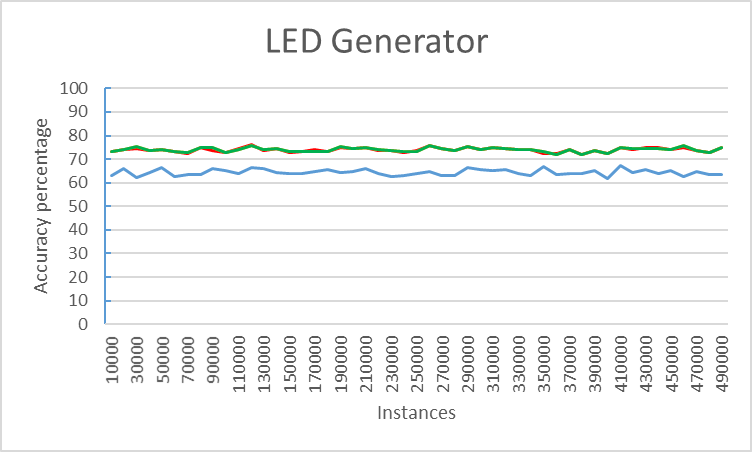
\includegraphics[scale=0.25]{Graphs/LED/10_graph}
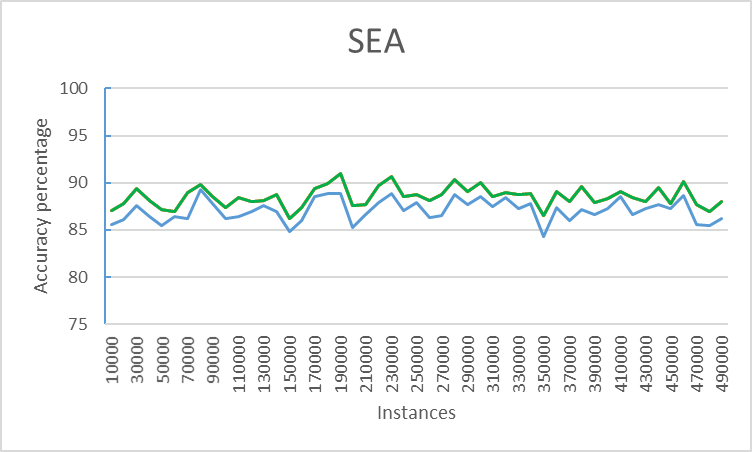
\includegraphics[scale=0.25]{Graphs/SEA/graph}
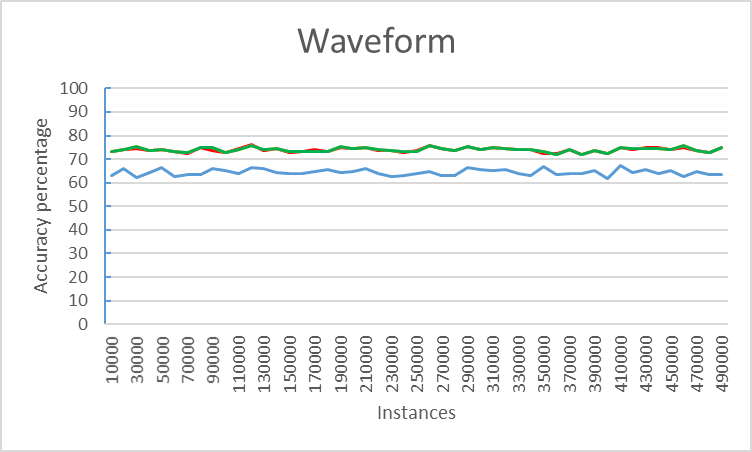
\includegraphics[scale=0.25]{Graphs/Waveform/graph}
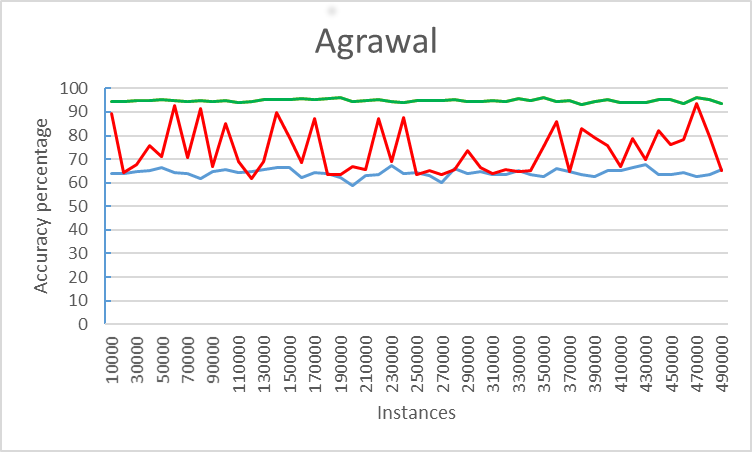
\includegraphics[scale=0.25]{Graphs/Agrawal/graph}
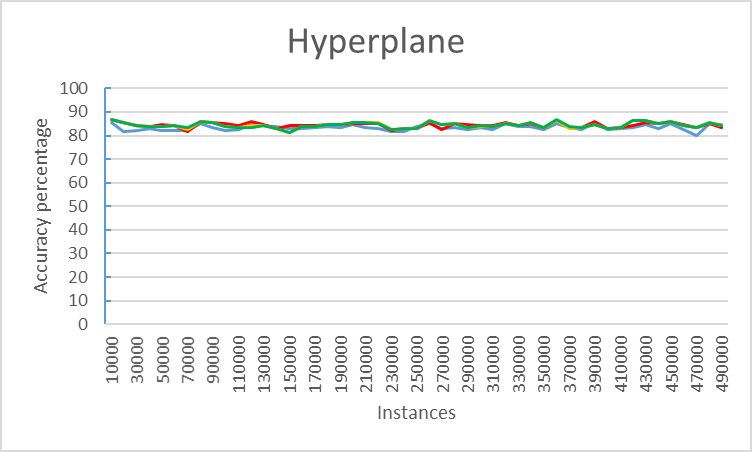
\includegraphics[scale=0.25]{Graphs/Hyperplane/graph}
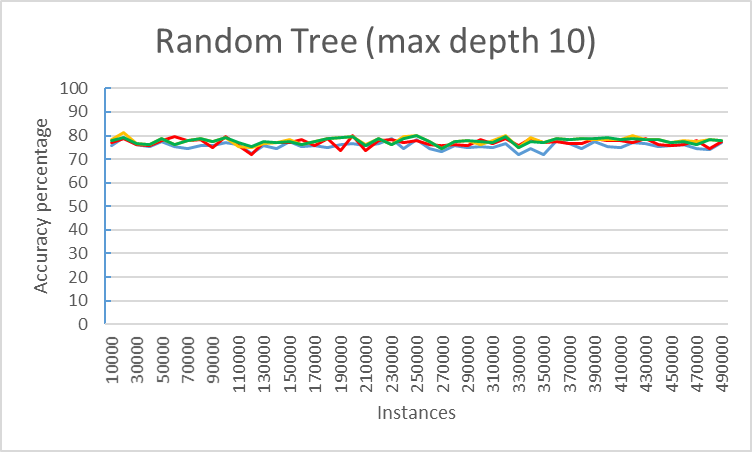
\includegraphics[scale=0.25]{Graphs/TreeD10/graph}
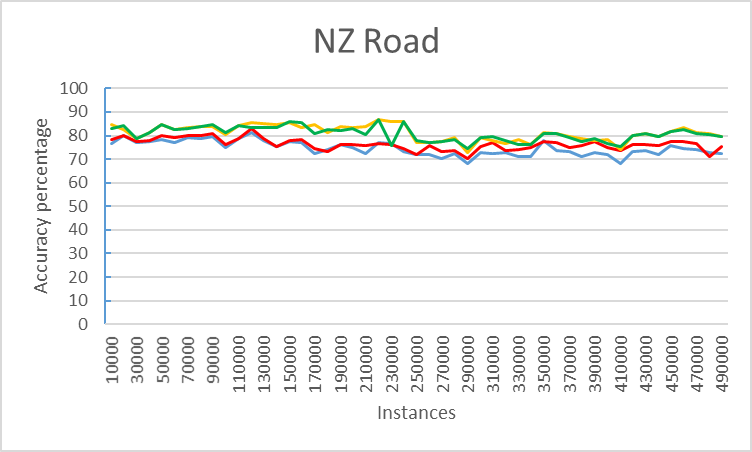
\includegraphics[scale=0.25]{Graphs/NZRoad/graph}

\includegraphics[scale=0.5]{Graphs/legend}
\caption{Prediction Accuracy for static $f$. Lines overlap for some graphs.}
\label{fig:graphs1}
\end{center}
\end{figure}

% fy graphs
\begin{figure}[h]
\begin{center}
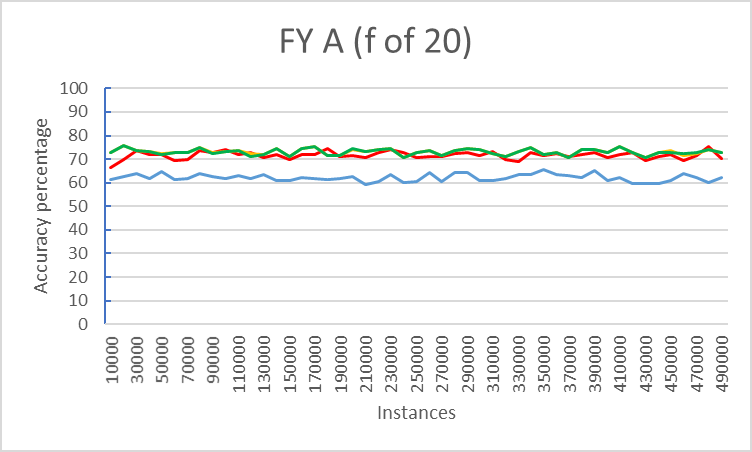
\includegraphics[scale=0.25]{Graphs/FY_A/graph20}
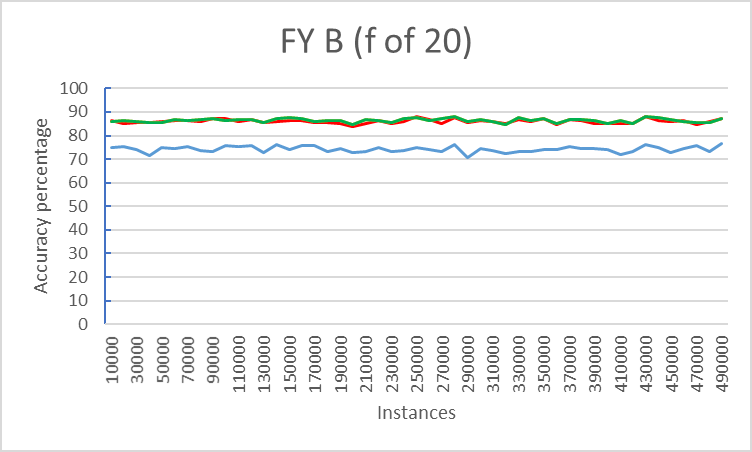
\includegraphics[scale=0.25]{Graphs/FY_B/graph20}
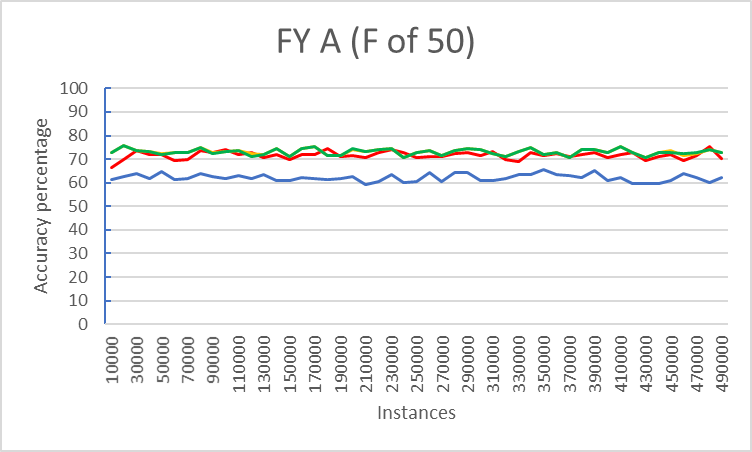
\includegraphics[scale=0.25]{Graphs/FY_A_Drift/graph}
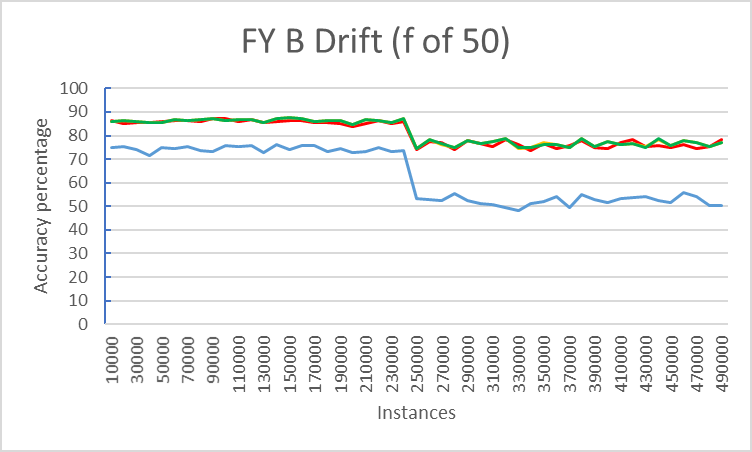
\includegraphics[scale=0.25]{Graphs/FY_B_Drift/graph}
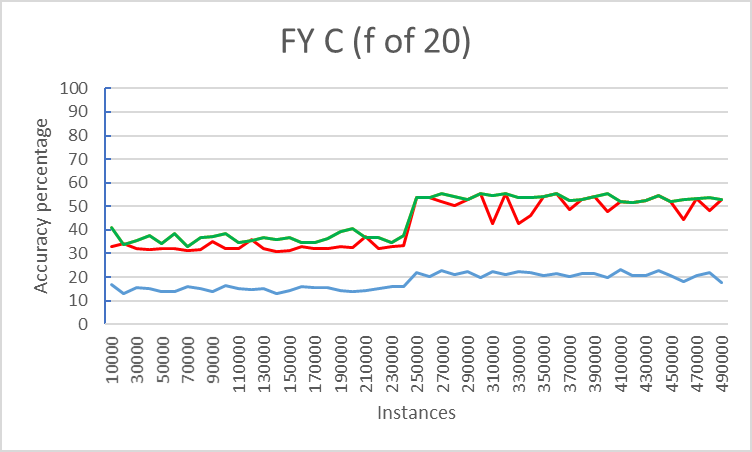
\includegraphics[scale=0.25]{Graphs/FY_C/graph20}
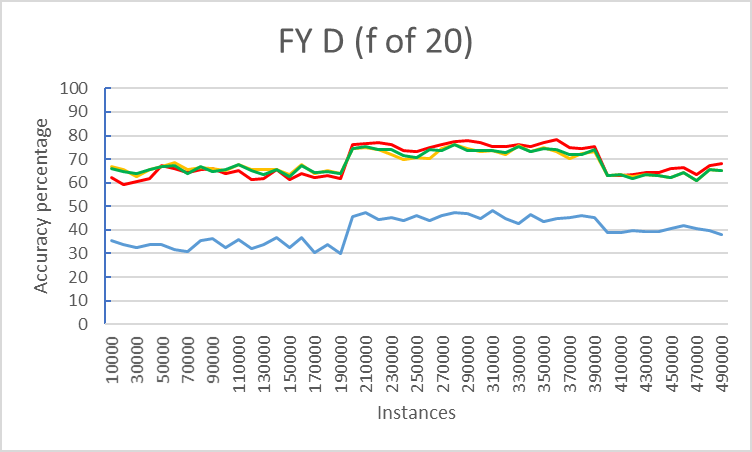
\includegraphics[scale=0.25]{Graphs/FY_D/graph20}

\includegraphics[scale=0.5]{Graphs/legend}
\caption{Prediction accuracy for static $f$.}
\label{fig:graphs2}
\end{center}
\end{figure}

\begin{figure}[h]
\begin{center}
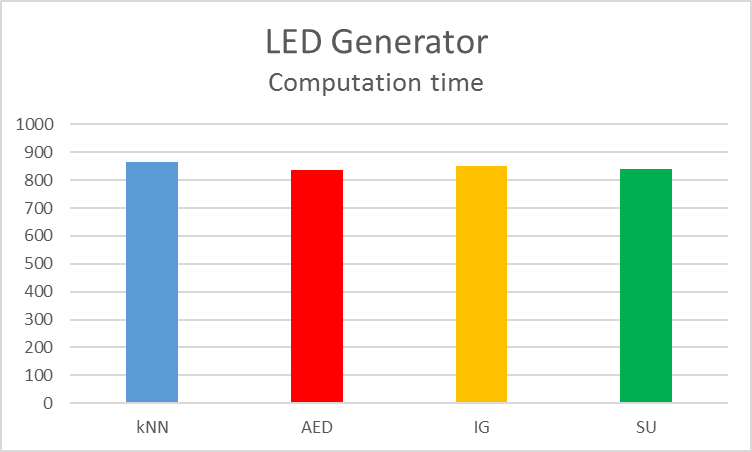
\includegraphics[scale=0.17]{Graphs/LED/10_time}
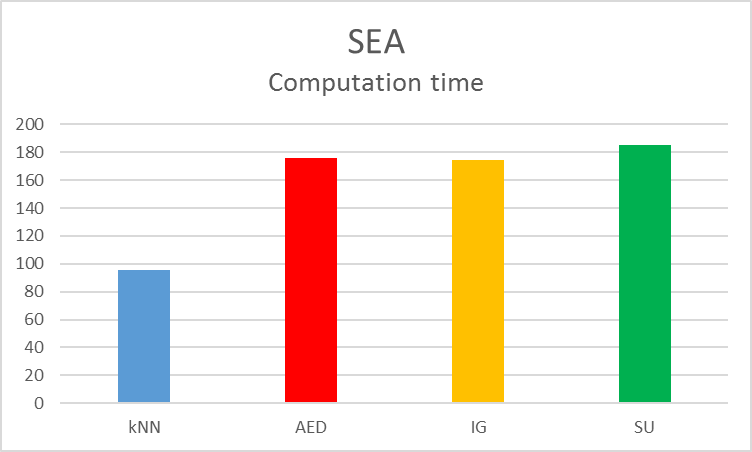
\includegraphics[scale=0.17]{Graphs/SEA/time}
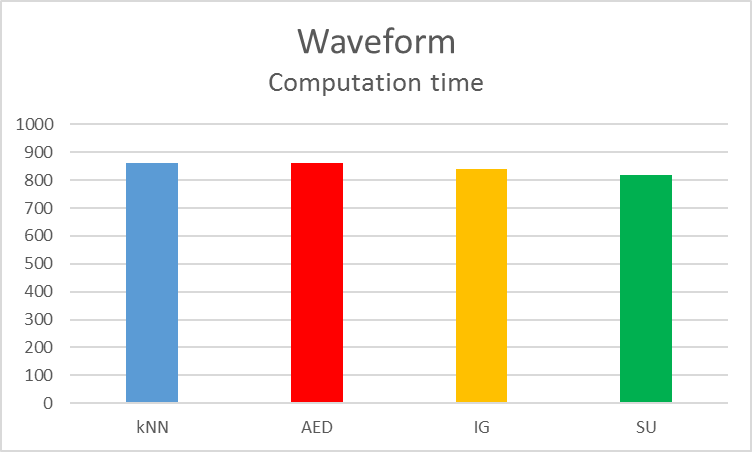
\includegraphics[scale=0.17]{Graphs/Waveform/time}
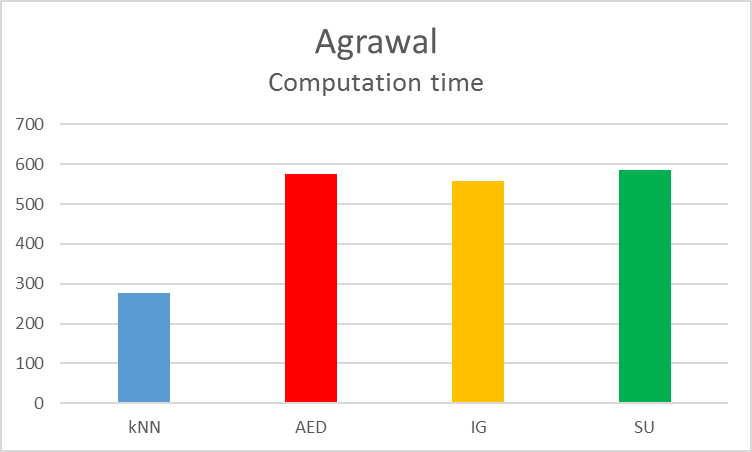
\includegraphics[scale=0.17]{Graphs/Agrawal/time}
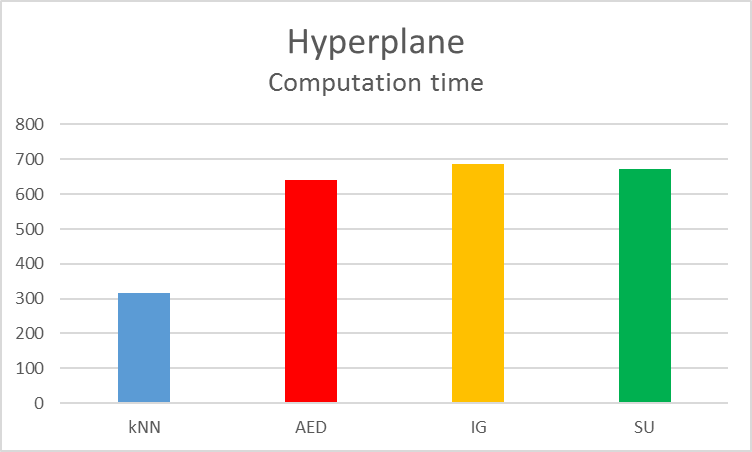
\includegraphics[scale=0.17]{Graphs/Hyperplane/time}
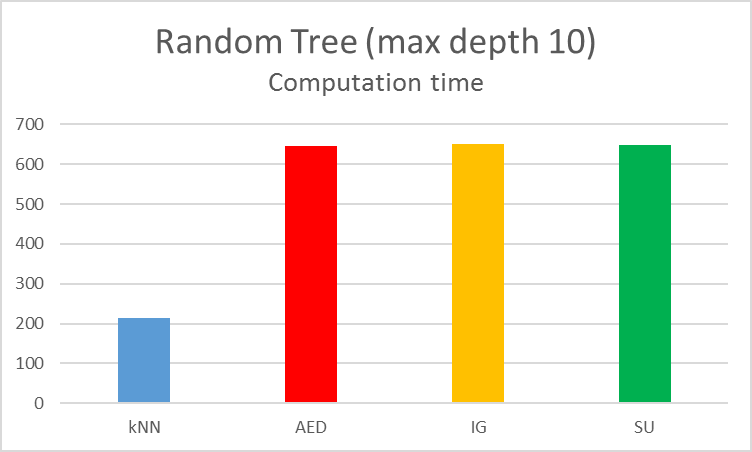
\includegraphics[scale=0.17]{Graphs/TreeD10/time}
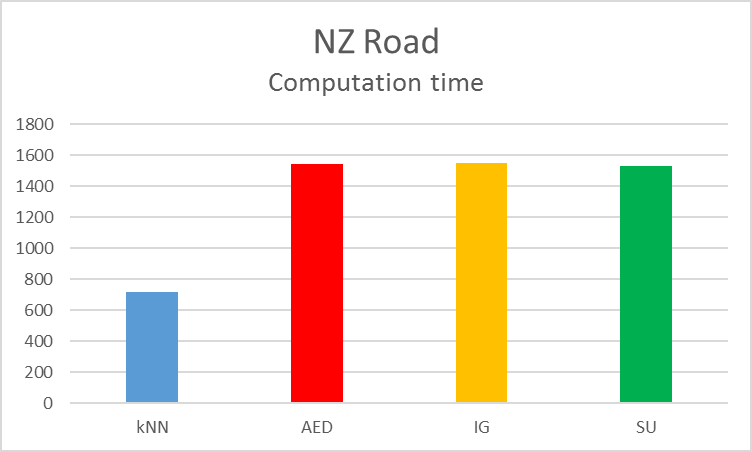
\includegraphics[scale=0.17]{Graphs/NZRoad/time}
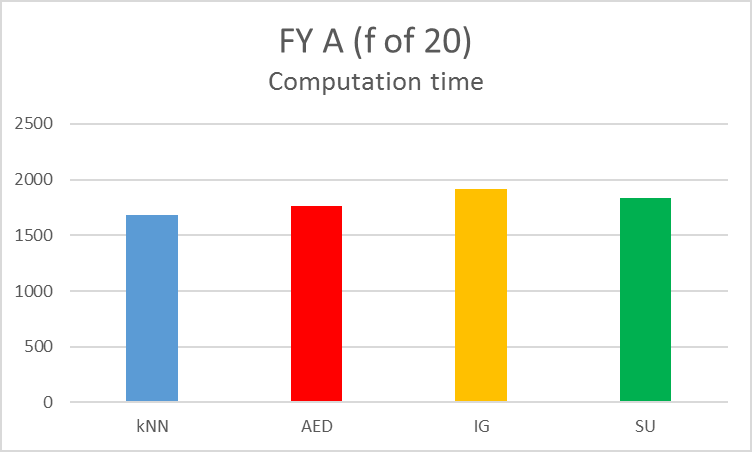
\includegraphics[scale=0.17]{Graphs/FY_A/time20}
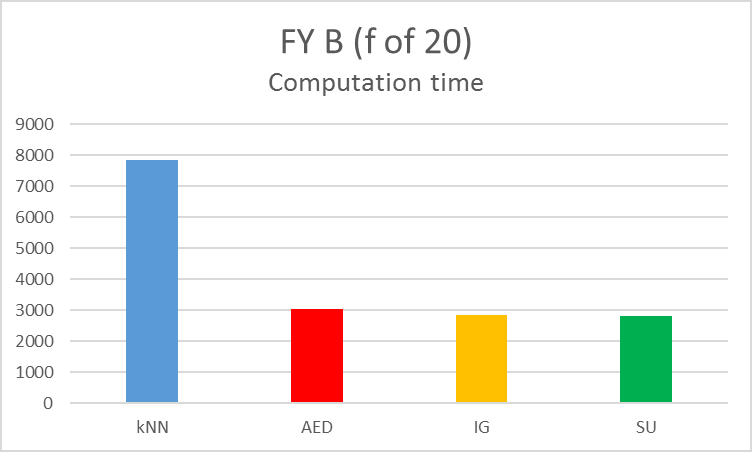
\includegraphics[scale=0.17]{Graphs/FY_B/time20}
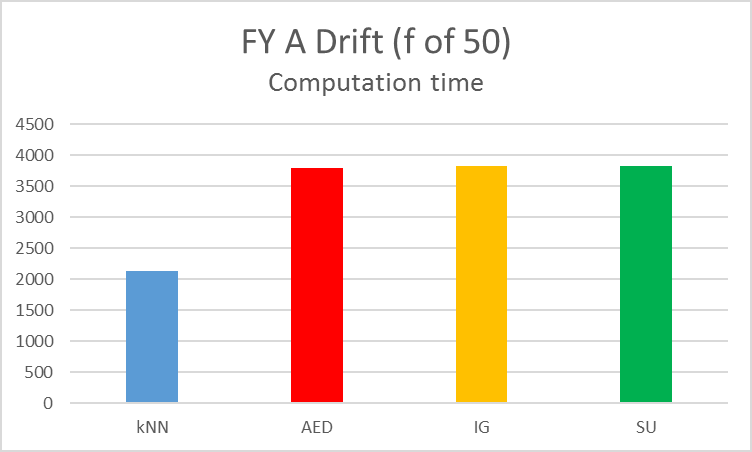
\includegraphics[scale=0.17]{Graphs/FY_A_Drift/time}
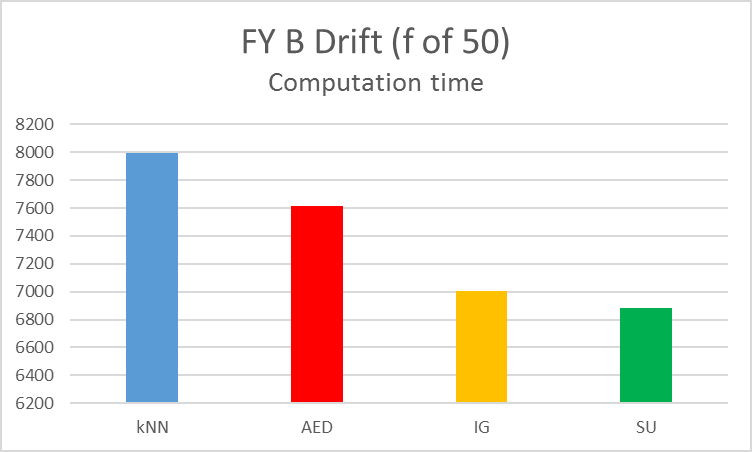
\includegraphics[scale=0.17]{Graphs/FY_B_Drift/time}
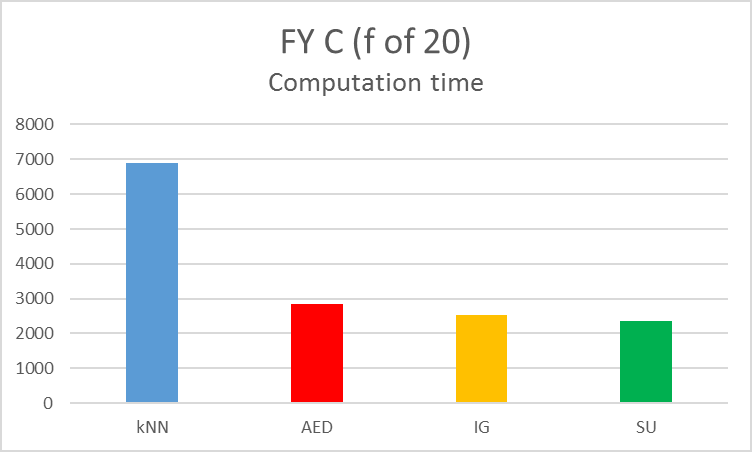
\includegraphics[scale=0.17]{Graphs/FY_C/time20}
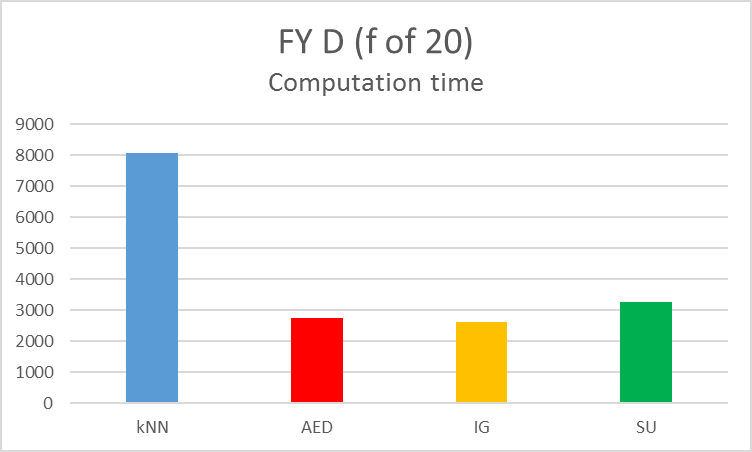
\includegraphics[scale=0.17]{Graphs/FY_D/time20}
\caption{Computation time in seconds of static $f$ experiments.}
\label{fig:time}
\end{center}
\end{figure}

Figure \ref{fig:graphs1} contains prediction accuracy plotted over the stream as new examples come in for static $f$ experiments. Improvements in prediction accuracy can be observed across all experiments when comparing the kNN without feature selection to kNN with feature selection so long as a $f$ of sufficient size was selected. This holds for streams with both a high and low number of features. It was found that selecting a static $f$ too small is detrimental to prediction accuracy as too many features are culled from feature selection, in some cases resulting in worse accuracy than kNN without feature selection. The three ranking functions gave mostly similar results, with SU tending to perform slightly better on average than the other two ranking functions in terms of overall classification accuracy, though not by much. IG and SU ranking functions for the most part performed very similarly to each other due to both being entropy based functions. On experiments such as the Hyperplane and Random tree, the IG and SU lines almost completely overlap each other when plotted on a graph.

In streams without completely irrelevant features such as the Hyperplane and Random tree generators, feature selection was still able to perform with mean accuracies on par with kNN without feature selection so long as $f$ was selected to cover the whole stream. In some cases, very slight improvements (less than 1\%) in mean accuracy were observed for some experiments but were for the most part, marginal and mostly irrelevant. In streams with more irrelevant features, improvement in prediction accuracy over kNN without feature selection is more pronounced. We observed an improvement of roughly 10\% over kNN without feature selection at all times in the LED, Waveform, FY A, and FY B experiments. In the more complex streams (FY C and FY D), very significant improvements were observed with feature selection performing around 30\% better than kNN without feature selection. We also observed that in streams with sudden concept change such as the FY A Drift, FY B Drift, FY C and FY D data sets, the improvement of kNN with feature selection over kNN without feature selection stayed consistent despite drift.

Drifting feature ordering was also tested in the form of the LED Drift and Waveform Drift generators which gave almost identical results to the generators without drift, and hence were not included in graphs. It does however indicate that the feature selection and ranking functions are robust against movements of features' position in the feature space and not biased towards features based on their position in the stream.

Figure \ref{fig:time} shows the time it took for each experiment to complete in seconds. Computation time was found to be highly dependent on the $f$ parameter and how close $f$ is to the actual number of relevant features. How well the ranking function is able to identify the relevant features from the irrelevant features is also important as it impacts on how close $f$ can be set to the actual number of relevant features.

For static $f$ experiments, when $f$ is set close to the actual number of relevant features in a stream with at least some irrelevant features such as in the LED, Waveform, and Conditional generator experiments (FY A, FY B, FY C, and FY D), feature selection outperforms kNN without feature selection in terms of computation time as seen in \ref{fig:time}. This gap widens as the ratio of relevant to irrelevant features increases. In complex streams with more irrelevant features than relevant features as in the FY B, FY C, and FY D, computation time for the best ranking function is around 1/3 that of kNN without feature selection which is a very significant improvement. The three ranking functions had relatively similar computation times, with the AED ranking function seemingly performing faster than the IG and SU ranking functions in streams with more nominal features (such as the SEA and LED experiments) while IG and SU seems to perform faster than AED in streams with more numeric features (such as the Waveform and Hyperplane experiments). Overall, streams with more numeric attributes tended to take longer to compute than those with only nominal attributes due to the added overhead of discretisation for IG and SU, or calculating the mean for AED.

Memory wise, feature selection uses slightly more memory than kNN. The difference is small however with on average 3-6\% increase for the serialised model size. The difference in memory usage is also tied to the types of features in the stream (whether they are nominal or numeric), the features' complexity, and the number of irrelevant features in the stream. The size of $f$ also has an impact on memory usage but the impact is mostly negligible; for example, the experiment on the LED generator used 40 more bytes to construct its model for a $f$ of 20 compared to a $f$ of 10. IG and SU ranking function take the same amount of memory to construct their model in all experiments tested, and tended to in most cases use slightly less memory than the AED ranking function.

\section{Hill climbing $f$ for dynamic subset size selection}

\begin{figure}[h]
\begin{center}
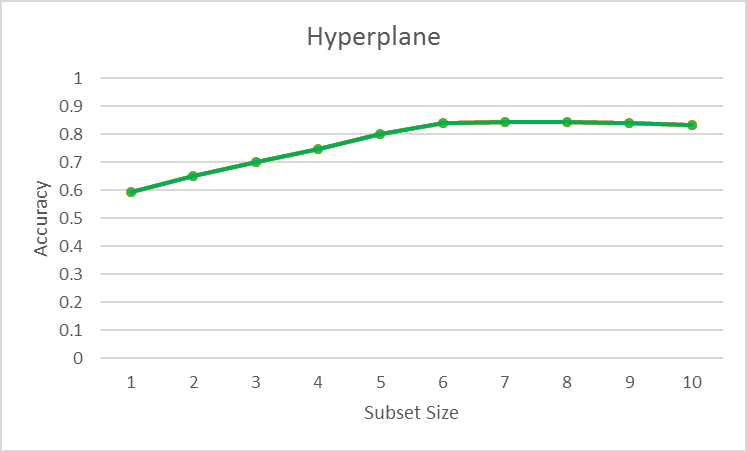
\includegraphics[scale=0.25]{Graphs/AccuracyDifference/Hyperplane}
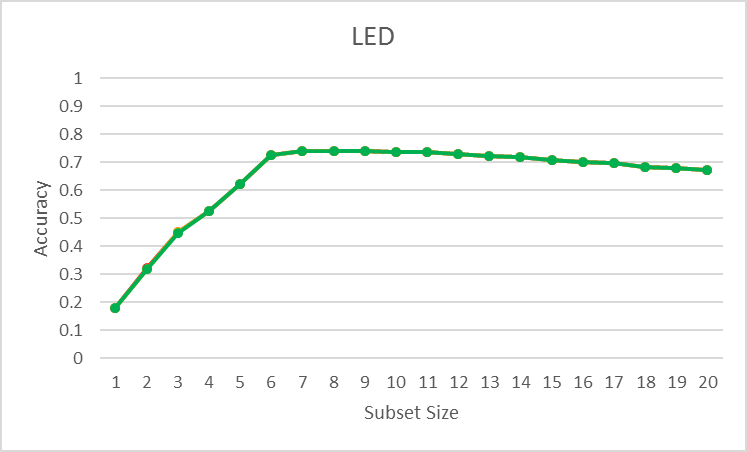
\includegraphics[scale=0.25]{Graphs/AccuracyDifference/LED20}
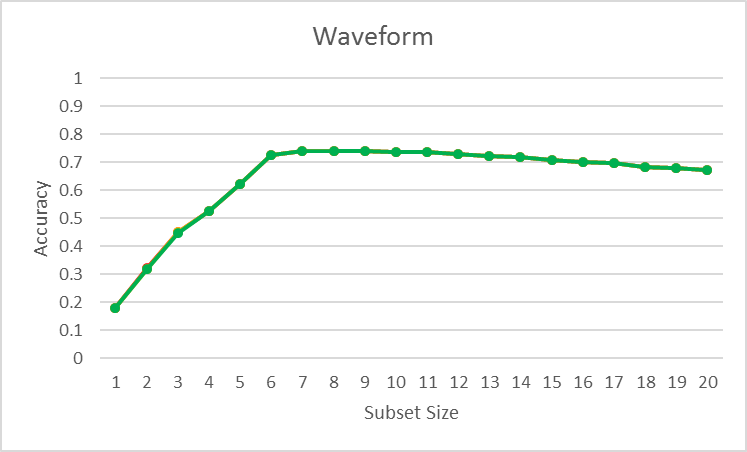
\includegraphics[scale=0.25]{Graphs/AccuracyDifference/Waveform}
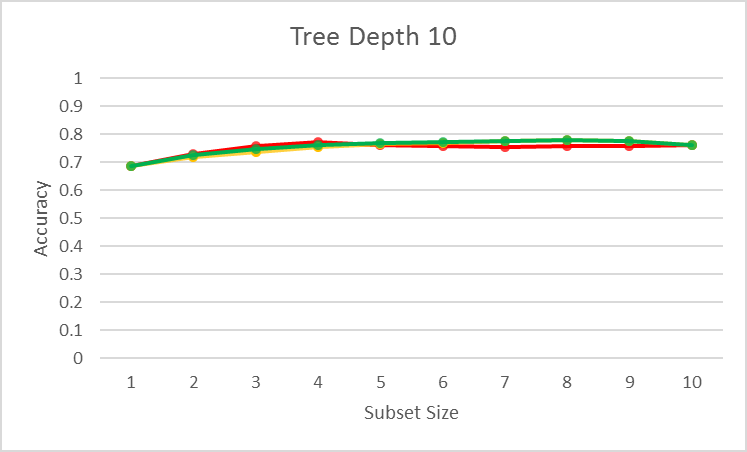
\includegraphics[scale=0.25]{Graphs/AccuracyDifference/TreeD10}
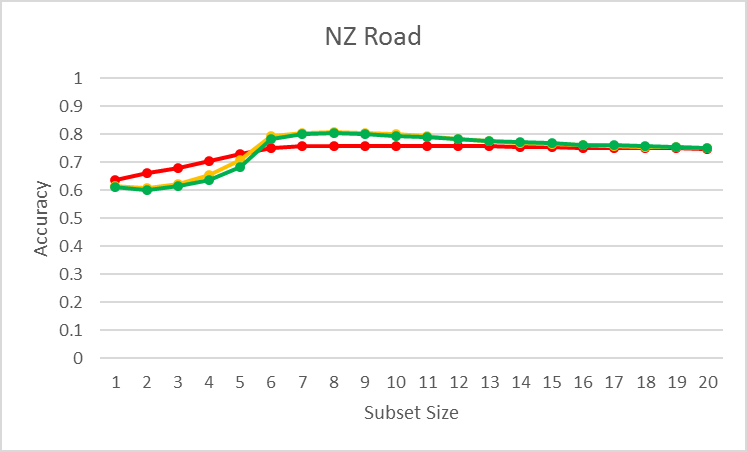
\includegraphics[scale=0.25]{Graphs/AccuracyDifference/NZRoad20}
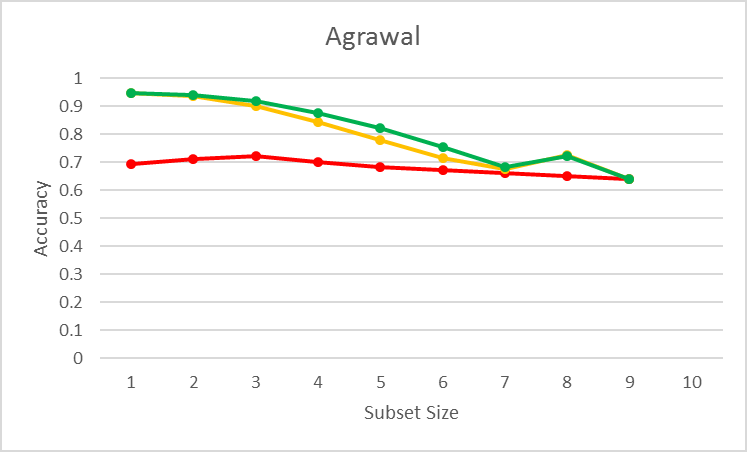
\includegraphics[scale=0.25]{Graphs/AccuracyDifference/Agrawal}
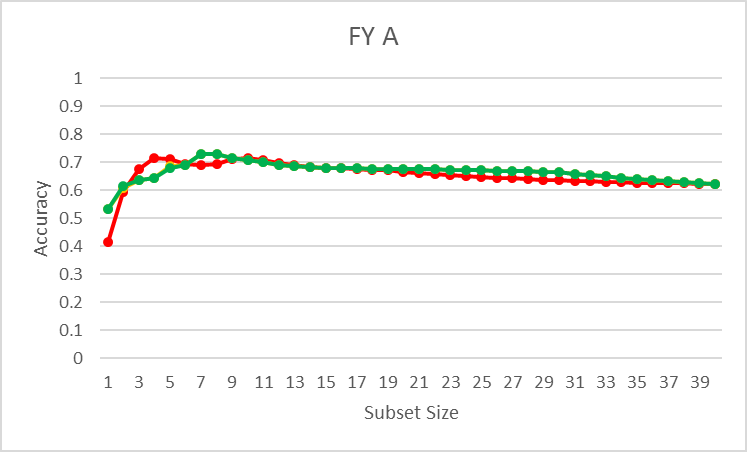
\includegraphics[scale=0.25]{Graphs/AccuracyDifference/FY_A}
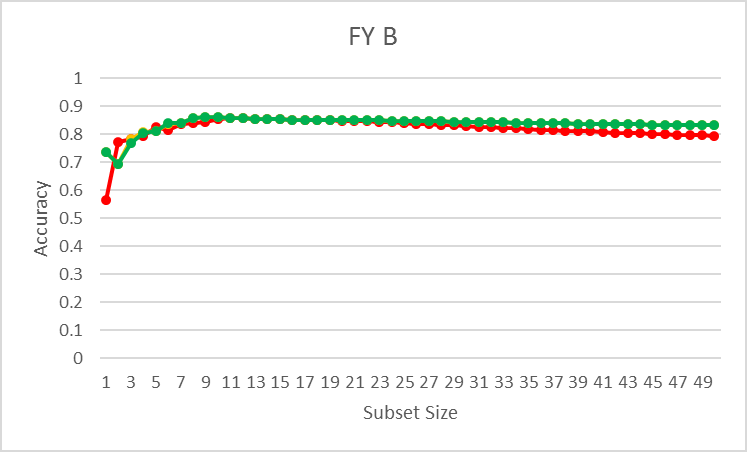
\includegraphics[scale=0.25]{Graphs/AccuracyDifference/FY_B}

\includegraphics[scale=0.5]{Graphs/legendNokNN}
\caption{Average accuracy difference as subset size increases. Lines overlap on some graphs, hence showing only one line.}
\label{fig:accuracyDifference}
\end{center}
\end{figure}

\begin{figure}[h]
\begin{center}
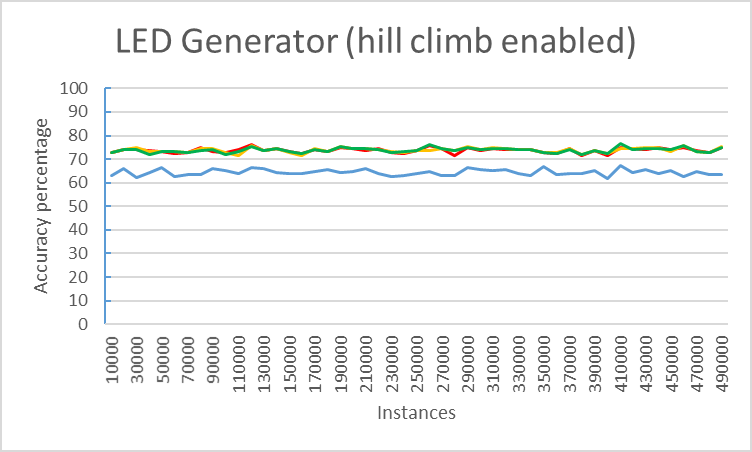
\includegraphics[scale=0.25]{Graphs/LED/H_graph}
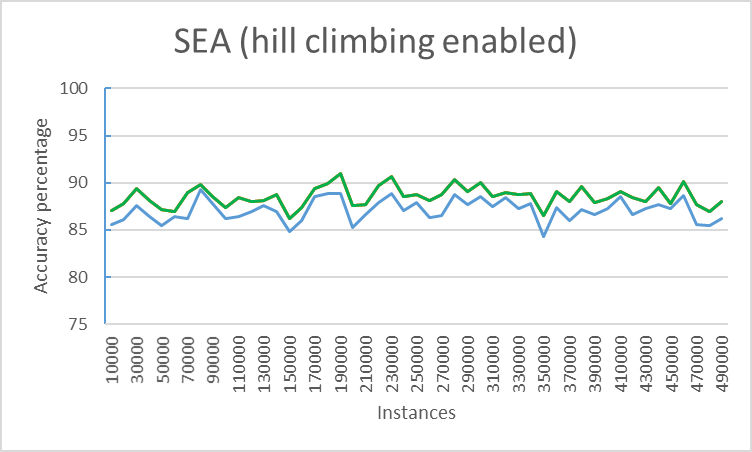
\includegraphics[scale=0.25]{Graphs/SEA/H_graph}
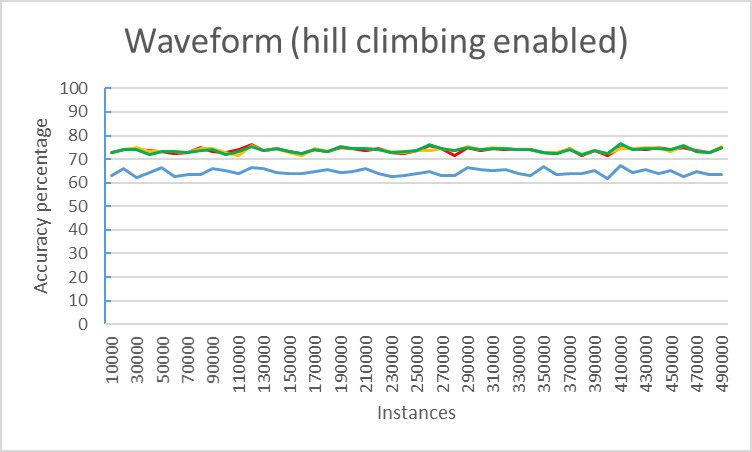
\includegraphics[scale=0.25]{Graphs/Waveform/H_graph}
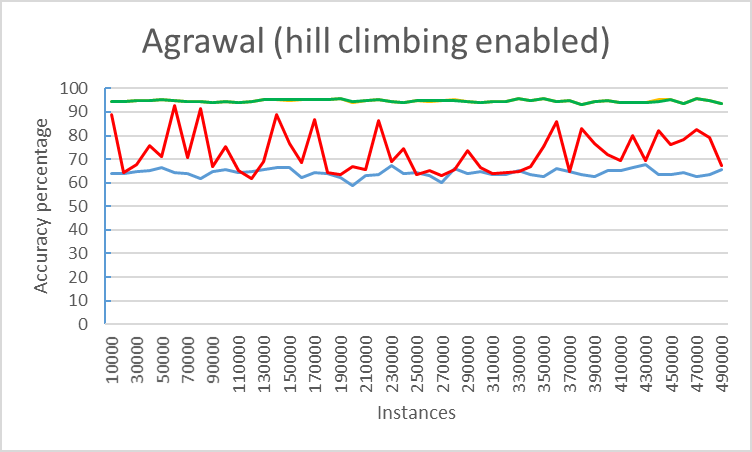
\includegraphics[scale=0.25]{Graphs/Agrawal/H_graph}
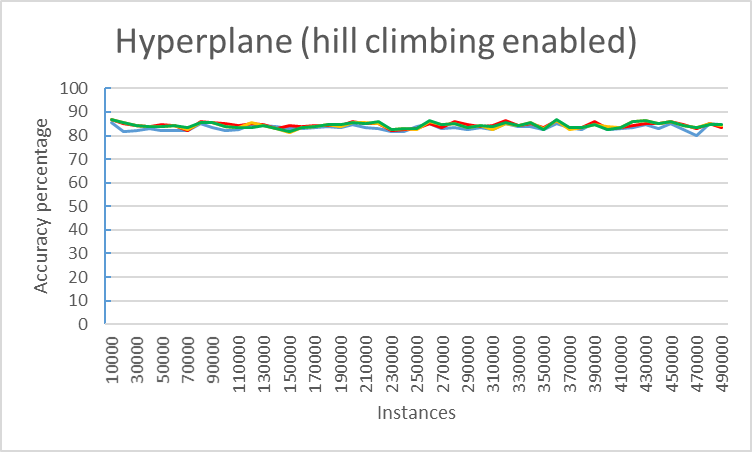
\includegraphics[scale=0.25]{Graphs/Hyperplane/H_graph}
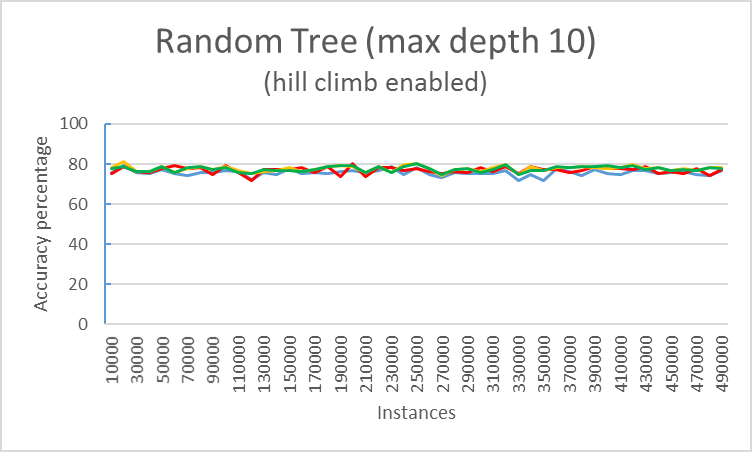
\includegraphics[scale=0.25]{Graphs/TreeD10/H_graph}
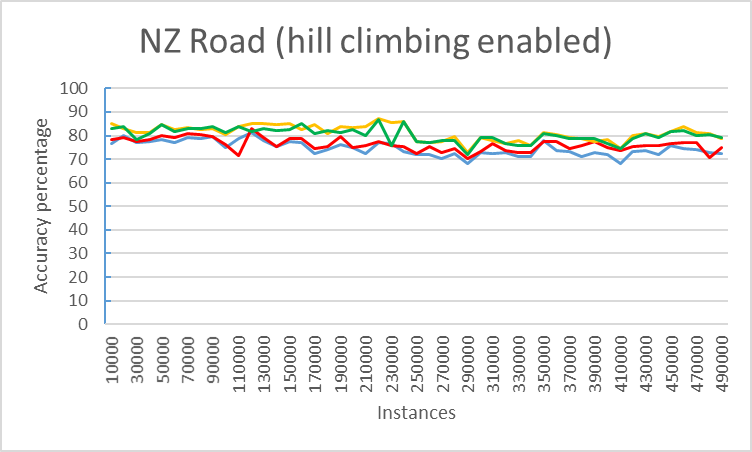
\includegraphics[scale=0.25]{Graphs/NZRoad/H_graph}

\includegraphics[scale=0.5]{Graphs/legend}
\caption{Prediction accuracy for experiments with hill climbing enabled on data streams with a low (less 30) number of features. Lines overlap on some graphs.}
\label{fig:graphs_h}
\end{center}
\end{figure}

\begin{figure}[h]
\begin{center}
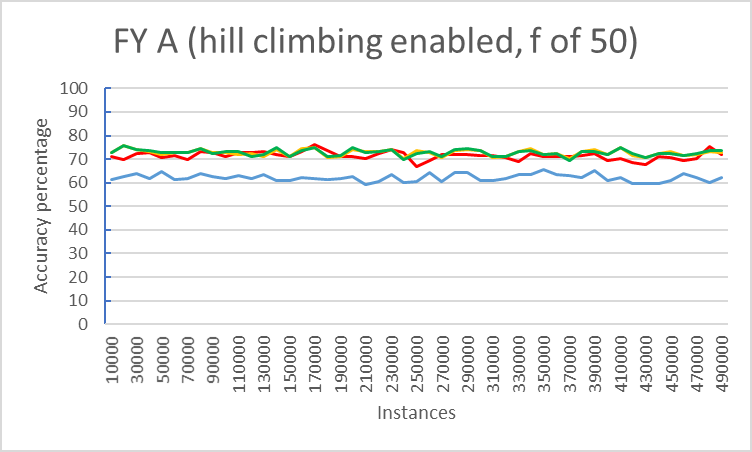
\includegraphics[scale=0.25]{Graphs/FY_A/H_graph}
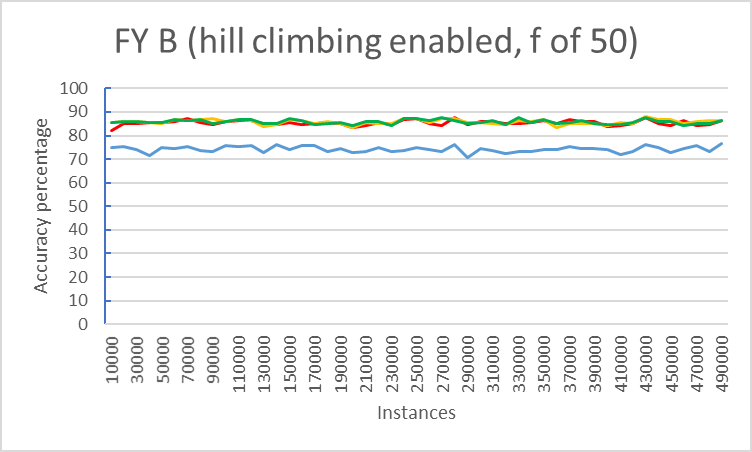
\includegraphics[scale=0.25]{Graphs/FY_B/H_graph}
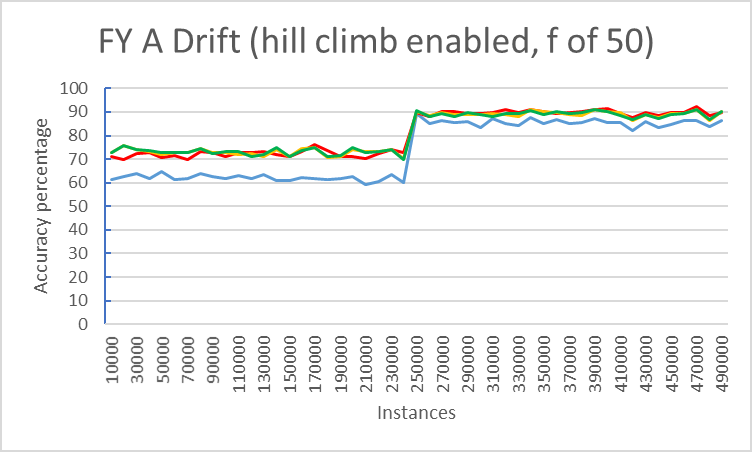
\includegraphics[scale=0.25]{Graphs/FY_A_Drift/H_graph}
\includegraphics[scale=0.25]{Graphs/FY_B_Drift/H_graph}
\includegraphics[scale=0.25]{Graphs/FY_C/H_graph}
\includegraphics[scale=0.25]{Graphs/FY_D/H_graph}
\includegraphics[scale=0.5]{Graphs/legend}
\caption{Prediction accuracy for experiments with hill climbing enabled on conditional generator data sets with a high number of features.}
\label{fig:graphs2_h}
\end{center}
\end{figure}



\begin{figure}[h]
\centering 
\includegraphics[scale=0.17]{Graphs/LED/H_time}
\includegraphics[scale=0.17]{Graphs/SEA/H_time}
\includegraphics[scale=0.17]{Graphs/Waveform/H_time}
\includegraphics[scale=0.17]{Graphs/Agrawal/H_time}
\includegraphics[scale=0.17]{Graphs/Hyperplane/H_time}
\includegraphics[scale=0.17]{Graphs/TreeD10/H_time}
\includegraphics[scale=0.17]{Graphs/NZRoad/H_time}
\includegraphics[scale=0.17]{Graphs/FY_A/H_time}
\includegraphics[scale=0.17]{Graphs/FY_B/H_time}
\includegraphics[scale=0.17]{Graphs/FY_A_Drift/H_time}
\includegraphics[scale=0.17]{Graphs/FY_B_Drift/H_time}
\includegraphics[scale=0.17]{Graphs/FY_C/H_time}
\includegraphics[scale=0.17]{Graphs/FY_D/H_time}
\caption{Computation time in seconds of hill climbing $f$ experiments.}
\label{fig:time_h}
\end{figure}

Figure \ref{fig:graphs_h} and \ref{fig:graphs2_h} show the prediction accuracy results for experiments where hill climbing was enabled to dynamically select $f$. In most experiments prediction accuracy suffered a slight decrease when compared to experiments where $f$ is static. The difference however is very small (around 1\% maximum) and generally not impactful. For the same size of $f$, the serialised model size was the same for hill climbing experiments and static $f$ experiments .



\begin{table}[h]
\centering
\begin{tabular}{r|rrr}
						   & No feature selection & Hill climbing $f$ & Static $f$  \\ \hline
LED                        & 863.667   & 616.677    & 840.849   \\
SEA                        & 95.7661   & 183.604    & 185.033   \\
Waveform                   & 862.715   & 613.143    & 818.568   \\
Agrawal                    & 277.674   & 208.513    & 586.588   \\
Hyperplane                 & 314.889   & 539.871    & 673.610   \\
Random Tree                & 214.071   & 488.963    & 649.401   \\
NZ Road                    & 716.659   & 1238.005   & 1533.165  \\
FY A                       & 1681.966  & 780.902    & 1835.689  \\
FY B                       & 7854.827  & 1502.846   & 2811.226  \\
FY A Drift                 & 2134.140  & 958.267    & 1885.345  \\
FY B Drift                 & 7998.333  & 1563.532   & 2743.101  \\
FY C                       & 6890.245  & 806.470    & 2345.209  \\
FY D                       & 8064.495  & 1505.151   & 3275.735 
\end{tabular}
\caption{Comparison of computation time for SU experiments using hill climbing to dynamically select $f$ versus experiments using a static $f$ and experiments with no feature selection.}
\label{Table:H_Time_v_Static}
\end{table}

Figure \ref{fig:time_h} and table \ref{Table:H_Time_v_Static} show the computation time for all experiments conducted. For streams with a highly fluctuating number of relevant features and/or a large number of irrelevant features, as in the FY A, FY B, FY C, and FY D data sets, we observed significant improvements for computation time compared to the static $f$ experiments. The improvement is especially impressive considering the hill climbing experiments had an upper bound of 50 features while the static $f$ experiments considered only the top 20 features, meaning we were able to cover a larger number of features using less time. For streams without many irrelevant features such as the Random tree and Hyperplane generators, hill climbing still performed similarly to static $f$ for computation time and memory usage.

A downside to hill climbing as previously mentioned, is the potential for the algorithm to become stuck in a local optima. If the ranking function was not able to correctly identify and rank the most relevant features above irrelevant features or features detrimental to accuracy, there is a possibility for local optimas to exist. If the hill climbing window is not sufficiently large enough to climb out of the local optimum, the algorithm may get stuck in a suboptimal subset size and prediction accuracy can suffer as a result. One such case can be observed in the FY B data set where the accuracy dips for the IG and SU ranking functions at a subset size of 2, creating a local optima of at subset 1 (This local optimum can be seen on figure \ref{fig:accuracyDifference}). In an extreme case where the hill climbing window is set to 1, the algorithm gets stuck on the local optimum of 1 and considers only one feature for the entire stream; the consequence of which can be seen in figure \ref{fig:stuck_graph}, where both the IG and SU ranking functions' prediction accuracies suffer greatly as a result. However, this is more of an edge case for the entropy based ranking functions and is not replicated in the AED ranking function. A hill climbing window of 2 also alleviates this problem and dislodges the algorithm from the local optima for the entropy based ranking functions. 

The problem still exists however, as simply enlarging the hill climbing window is not an elegant, nor reliable solution. A hill climbing window too large degenerates the algorithm to static $f$ and there is still potential for the algorithm to become stuck even with a very large hill climbing window, though we did not observe any such issue in the experiments we conducted with a hill climbing window of 2.

\begin{figure}[h]
\centering 
\includegraphics[scale=0.25]{Graphs/FY_B/H_graph_stuck}
\includegraphics[scale=0.5]{Graphs/legend}
\caption{FY B with a hill climbing window of 1.}
\label{fig:stuck_graph}
\end{figure}

Despite this potential for getting stuck, we conclude that hill climbing is almost always worth the slight drop in accuracy for the significant improvements in computation time.

\section{Different $k$ sizes}
\begin{table}[h]
\centering
\begin{tabular}{r|rrr}
            & ISS kNN 5 SU & ISS kNN 10 SU & ISS kNN 20 SU \\ \hline
LED         & 73.666   & 73.838    & 73.684    \\
SEA         & 88.012   & 88.514    & 88.554    \\
Waveform    & 73.666   & 73.838    & 73.684    \\
Agrawal     & 94.646   & 94.656    & 94.632    \\
Hyperplane  & 83.122   & 84.396    & 86.106    \\
Random Tree & 77.354   & 77.530    & 77.896    \\
NZ Road     & 80.156   & 80.440    & 80.348    \\
FY A        & 71.344   & 72.768    & 72.788    \\
FY B        & 85.612   & 85.870    & 85.864    \\
FY A Drift  & 80.312   & 81.078    & 80.782    \\
FY B Drift  & 80.442   & 80.804    & 81.522    \\
FY C        & 44.232   & 44.816    & 45.014    \\
FY D        & 66.536   & 67.560    & 68.774
\end{tabular}
\caption{Average prediction accuracy of feature selection using SU ranking with hill climbing enabled for various sizes of $k$.}
\label{Table:K_Table_Accuracy}
\end{table}

We tested our algorithm with different settings for the number of nearest neighbours $k$ to make sure our positive results for a $k$ of 10 was consistent with other sizes of $k$. Due to the constraints of time we only tested the SU ranking function with hill climbing enabled for with different $k$ sizes. $k$ sizes of 5, 10 and 20 were tested. For all sizes of $k$, feature selection continued to show improvements over kNN without feature selection. 

It was observed that overall, the size of $k$ makes a very marginal difference to average prediction accuracy when feature selection was enabled, with a less than 1\% difference in all cases tested. Computation time was somewhat variable in experiments and the results shown in table \ref{Table:K_Table_Time} are the mean computation time of 3 separate experiments for each $k$ size. The general trend observed was that a smaller $k$ tended to compute faster while giving slightly worse accuracy while a larger $k$ gave slightly better accuracy but computed slower. We observed that for some datasets, such as that of the FY B Drift and FY D experiments, the trend is much more pronounced than other experiments. A hypothesis of why this is the case is the different sizes of $k$ cause the hill climbing algorithm to select different sizes of $f$ on those datasets, in which case there would be slightly more or less computation depending on $f$. Memory usage was the same across all $k$ sizes and RAM hours followed the trend shown by computation time.

\begin{table}[h]
\centering
\begin{tabular}{r|rrr}                           
						   & kNN 5 SU & kNN 10 SU & kNN 20 SU \\  \hline
LED                        & 600.023  & 617.875   & 650.041  \\
SEA                        & 183.498  & 185.346   & 186.282  \\
Waveform                   & 600.786  & 620.163   & 649.7603  \\
Agrawal                    & 211.904  & 209.632   & 213.224  \\
Hyperplane                 & 527.956  & 542.545   & 569.375   \\
Random Tree                & 492.952  & 531.496   & 534.947  \\
NZ Road                    & 619.210  & 649.077   & 618.777  \\
FY A                       & 775.961  & 805.683   & 873.682  \\
FY B                       & 1683.483 & 1679.701  & 1849.045  \\
FY A Drift                 & 966.549  & 983.090   & 1055.164  \\
FY B Drift                 & 1487.486 & 1607.153  & 1707.508  \\
FY C                       & 793.588  & 833.257   & 865.196   \\
FY D                       & 1278.419 & 1511.023  & 1811.294
\end{tabular}
\caption{Mean computation time in seconds of feature selection using SU ranking with hill climbing enabled for various sizes of $k$.}
\label{Table:K_Table_Time}
\end{table}


\section{Adaptation to feature drift}
As mentioned in chapter \ref{chapter:RelatedWork}, previous studies have shown feature drift to negatively affect classifier performance in data streams, something feature selection can potentially help address. To test our method's ability to adapt to feature drift, we compared kNN with ISS feature selection to some well know classification algorithms used in stream mining in their ability to adapt to feature drifts. We conducted experiments on 4 data sets created using the Conditional Generator which all contain sudden feature drifts at the halfway point of the stream, except for the FY D dataset, which features two feature drifts at 200,000 and 400,000 instances. The algorithms tested were Naive Bayes (NB), the Hoeffding Tree (VFDT) \citep{Domingos:2000:MHD:347090.347107} and the Hoeffding Adaptive Tree (HAT) \citep{Bifet:2009:ALE:1617420.1617445}.

\begin{figure}[h]
\centering 
\includegraphics[scale=0.25]{Graphs/FeatureDrift/FY_A_Drift}
\includegraphics[scale=0.25]{Graphs/FeatureDrift/FY_B_Drift}
\includegraphics[scale=0.25]{Graphs/FeatureDrift/FY_C}
\includegraphics[scale=0.25]{Graphs/FeatureDrift/FY_D}
\includegraphics[scale=0.5]{Graphs/legendCompareFD}
\caption{Accuracy comparison of various classification algorithms over streams with sudden feature drifts.}
\label{fig:FeatureDrift}
\end{figure}

Figure \ref{fig:FeatureDrift} shows the different algorithms tested on datasets with feature drift. Overall, we observed that kNN based methods appeared to be more resilient to feature drift than the other the algorithms tested with no noticeable dips in accuracy. This is expected behaviour due to kNN's use of the sliding window which allows it to implicitly adapt to change. What is interesting is that ISS appears to amplify simplifications in the stream as seen in the FY C dataset, where after the occurrence of feature drift, the kNN algorithm's accuracy increases by roughly 5\% while the kNN with ISS algorithm's accuracy increases by around 15\%.


\begin{table}[h]
\centering
\begin{tabular}{r|rrr}
          & Mean accuracy & First concept & Second concept \\  \hline
kNN       & 73.876        & 62.132                      & 85.620                       \\
ISS SU HC & 81.078        & 72.988                      & 89.168                       \\
NB        & 79.502        & 87.352                      & 71.652                       \\
VFDT      & 88.110        & 86.740                      & 89.480                       \\
HAT       & 89.142        & 86.288                      & 91.996                      
\end{tabular}
\caption{Mean accuracies for FY A Drift dataset for various classification algorithms.}
\label{Table:Feature_Drift_FY_A_Drift}
\end{table}


\begin{table}[h]
\centering
\begin{tabular}{r|rrr}
          & Mean accuracy & First concept & Second concept \\ \hline
kNN       & 63.324        & 74.316                      & 52.332                       \\
ISS SU HC & 80.804        & 85.852                      & 75.756                       \\
NB        & 69.010        & 92.088                      & 45.932                       \\
VFDT      & 80.048        & 92.164                      & 67.932                       \\
HAT       & 89.184        & 91.988                      & 86.380                       
\end{tabular}
\caption{Mean accuracies for FY B Drift dataset for various classification algorithms.}
\label{Table:Feature_Drift_FY_B_Drift}
\end{table}

\begin{table}[h]
\centering
\begin{tabular}{r|rrr}
          & Mean accuracy & First concept & Second concept \\ \hline
kNN       & 18.020        & 14.928                      & 21.112                       \\
ISS SU HC & 44.816        & 36.012                      & 53.620                        \\
NB        & 40.708        & 47.280                      & 34.136                       \\
VFDT      & 25.486        & 39.356                      & 11.616                       \\
HAT       & 46.012        & 39.244                      & 52.780                       
\end{tabular}
\caption{Mean accuracies for FY C dataset for various classification algorithms.}
\label{Table:Feature_Drift_FY_C}
\end{table}

\begin{table}[h]
\centering
\begin{tabular}{r|rrrr}
          & Mean accuracy & First concept & Second concept & Third concept \\ \hline
kNN       & 39.546        & 33.635                      & 45.410                        & 39.640                       \\
ISS SU HC & 67.560         & 64.085                      & 73.345                       & 62.940                       \\
NB        & 62.036        & 85.580                       & 54.080                        & 30.860                       \\
VFDT      & 42.466        & 76.915                      & 22.390                        & 13.720                       \\
HAT       & 75.822        & 75.730                       & 77.585                       & 72.480                      
\end{tabular}
\caption{Mean accuracies for FY D dataset for various classification algorithms.}
\label{Table:Feature_Drift_FY_D}
\end{table}

Results shown in tables \ref{Table:Feature_Drift_FY_A_Drift}, \ref{Table:Feature_Drift_FY_B_Drift}, \ref{Table:Feature_Drift_FY_C} and \ref{Table:Feature_Drift_FY_D} indicate that in the datasets tested, only the HAT algorithm had similar or better mean prediction accuracies compared to kNN with ISS feature selection; even then the HAT algorithm still exhibits noticeable drops in accuracy for datasets with many irrelevant features such as FY C and FY D. In both cases HAT drops below kNN with ISS after the occurrence of feature drift and takes around 50,000 examples to fully recover to a stable accuracy. 

An interesting observation was that algorithms which outperformed kNN with ISS before the feature drift, such as NB and VFDT, had worse or similar accuracies overall due to the dips in accuracy caused by feature drifts. In the FY D dataset, VFDT's prediction accuracy in fact never manages to stabilise nor recover, and ends with a 13\% prediction accuracy which is very close to the expected value for random guessing (10\%). We also observed that the kNN based algorithms (kNN without feature selection and kNN with ISS) adapted and stabilised much faster than the other algorithms after the occurrence of feature drift, which indicates that the implicit adaptation to feature drift offered by kNN through the use of a sliding window can be advantageous and faster than explicit adaptation in certain data streams.

We can conclude from these results that at least for the data sets tested, ISS  does aid in dealing with feature drifts and is able to make the simple and relatively poor performing kNN algorithm much more competitive with other stream classification algorithms while keeping the advantages of the kNN algorithm in feature drifting streams with many irrelevant features.

\section{Comparison to DFW}
\begin{figure}[h]
\centering 
\includegraphics[scale=0.17]{Graphs/LED/vsDFW}
\includegraphics[scale=0.17]{Graphs/SEA/vsDFW}
\includegraphics[scale=0.17]{Graphs/Waveform/vsDFW}
\includegraphics[scale=0.17]{Graphs/Agrawal/vsDFW}
\includegraphics[scale=0.17]{Graphs/Hyperplane/vsDFW}
\includegraphics[scale=0.17]{Graphs/TreeD10/vsDFW}
\includegraphics[scale=0.17]{Graphs/NZRoad/vsDFW}
\includegraphics[scale=0.17]{Graphs/FY_A/vsDFW}
\includegraphics[scale=0.17]{Graphs/FY_B/vsDFW}
\includegraphics[scale=0.17]{Graphs/FY_A_Drift/vsDFW}
\includegraphics[scale=0.17]{Graphs/FY_B_Drift/vsDFW}
\includegraphics[scale=0.17]{Graphs/FY_C/vsDFW}
\includegraphics[scale=0.17]{Graphs/FY_D/vsDFW}
\includegraphics[scale=0.5]{Graphs/legend2}
\caption{Prediction accuracy of kNN with ISS, kNN with DFW and kNN without feature selection.}
\label{fig:Accuracy_comparason}
\end{figure}

As an aside, we also compared ISS to Dynamic Feature Weighing (DFW). DFW is an algorithm proposed in \citep{Barddal:2016} which uses feature weighing to attempt to address feature drifts in streams. For our experiments, kNN with DFW was configured with a $k$ of 10 and window size of 1000, which is the same for what is used in the experiments for kNN with ISS and kNN without feature selection.

Overall, we observed that ISS performs much better than DFW on the datasets which were tested for this project. We observed better accuracies for ISS over all experiments at almost all points of the streams as shown in figure  \ref{fig:Accuracy_comparason}.

\begin{table}[h]
\centering
\begin{tabular}{r|rrr}
            & ISS SU HC kNN & DFW kNN 10 & kNN    \\ \hline
LED         & 73.838           & 60.630     & 64.404 \\
SEA         & 88.514           & 87.186     & 87.064 \\
Waveform    & 73.838           & 60.630     & 64.404 \\
Agrawal     & 94.656           & 69.442     & 64.194 \\
Hyperplane  & 84.396           & 83.704     & 83.424 \\
Random Tree & 77.530           & 75.690     & 75.690 \\
NZ Road     & 80.440           & 74.774     & 74.656 \\
FY A        & 72.768           & 62.952     & 62.182 \\
FY B        & 85.870           & 75.122     & 74.222 \\
FY A Drift  & 81.078           & 74.864     & 73.876 \\
FY B Drift  & 80.804           & 64.888     & 63.324 \\
FY C        & 44.816           & 18.100     & 18.020 \\
FY D        & 67.560           & 40.270     & 39.546
\end{tabular}
\caption{Average prediction accuracy of kNN with ISS versus kNN with DFW and kNN without feature selection.}
\label{Table:Accuracy_comparason}
\end{table}


\begin{table}[h]
\centering
\begin{tabular}{r|rrr}
            & ISS SU HC kNN & DFW kNN 10 & kNN         \\ \hline
LED         & 616.677          & 1464.050   & 863.667  \\
SEA         & 188.838          & 125.304    & 95.766   \\
Waveform    & 613.143          & 1429.401   & 862.715  \\
Agrawal     & 208.513          & 482.765    & 277.674  \\
Hyperplane  & 539.871          & 482.590    & 314.889  \\
Random Tree & 488.963          & 428.656    & 214.071  \\
NZ Road     & 675.980          & 1238.353   & 716.659  \\
FY A        & 780.902          & 3582.565   & 1681.966 \\
FY B        & 1502.846         & 14999.910  & 7854.827 \\
FY A Drift  & 958.267          & 3647.793   & 2134.140 \\
FY B Drift  & 1563.532         & 14837.190  & 7998.333 \\
FY C        & 806.470          & 13570.790  & 6890.245 \\
FY D        & 1505.151         & 15525.580  & 8064.495

\end{tabular}
\caption{Total computation time of kNN with ISS versus kNN with DFW and kNN without feature selection.}
\label{Table:Time_comparason}
\end{table}

Table \ref{Table:Time_comparason} shows the total computation times for ISS with hill climbing enabled using the SU ranking function versus DFW kNN and kNN without feature selection. It was observed that ISS was faster than DFW kNN in all experiments which contained irrelevant features except the SEA dataset. DFW kNN was also faster for the Hyperplane and Random Tree experiments, which had no irrelevant features. In terms of memory, ISS and DFW kNN had similar usage overall with DFW using around 3.2\% less memory on average based on the results of our experiments which can be seen in table \ref{Table:Mem_comparason}.

\begin{table}[h]
\centering
\begin{tabular}{r|rr}

            & ISS kNN & DFW kNN \\ \hline
LED         & 1481432          & 1450912    \\
SEA         & 441792           & 414096     \\
Waveform    & 1481432          & 1450912    \\
Agrawal     & 686568           & 655416     \\
Hyperplane  & 728096           & 695328     \\
Random Tree & 725696           & 695408     \\
NZ Road     & 1246024          & 1210040    \\
FY A        & 2166616          & 2113976    \\
FY B        & 6245448          & 6139272    \\
FY A Drift  & 2166616          & 2113976    \\
FY B Drift  & 6245448          & 6139272    \\
FY C        & 5839656          & 5648528    \\
FY D        & 6441816          & 6228840 

\end{tabular}
\caption{Serialised model size of kNN with ISS versus kNN with DFW and kNN without feature selection.}
\label{Table:Mem_comparason}
\end{table}





%----------------------------------------------------------------------------------------
%	SECTION 7
%----------------------------------------------------------------------------------------
\chapter{Conclusion}
\label{chapter:Conclusion}

We have presented an iterative and feature drift adaptive algorithm for feature selection in a stream setting. Our results indicate that feature selection does indeed have benefits to classification and computation time in data streams. As established in chapter \ref{chapter:Results}, the proposed feature selection method shows improvement for kNN classification accuracy and computation time in data streams with irrelevant features. We also were able to obtain classification accuracies as good or better than kNN without feature selection for data streams without irrelevant features, indicating that the algorithm is unlikely to actively hinder classifier performance. Our method was also able to adapt to feature drift faster than many of the other commonly used classification algorithms in stream mining. As our proposed method is a relatively simple method specialised for the kNN classifier, the promising results obtained from our experiments lead us to believe that feature selection in stream mining has great viability and potential in addressing the constraints of the stream setting and is definitely an area of interest for further study.

Due to the constraints of time some ideas were not fully explored, implemented or tested in the project.

A limitation we faced in our investigation was the lack of real world stream datasets. While synthetic data can to an extent simulate real world problems, underlying relationships between features in real world data are often times more complex than that of synthesised data; therefore it would be of interest to see how the algorithm performs in real world data sets. Feature drift was only tested on data sets from one generator as we lacked other datasets and gradual feature drift was also not tested due to a lack of data. Further expansion on the generator to implement a gradual feature drift could be something to look into.

Using Naive Bayes as the classifier algorithm over kNN is something that can be explored. As NB makes independent Bayesian predictions for each attribute, adding new attributes to the classifier to make a new prediction is extremely cheap. This potentially allows the algorithm to cover all features which would remove the need for hill climbing and perhaps even $f$.

The kNN classifier implementation can potentially be improved as it is currently rather slow. The main issue of our implementation is the performance cost of finding the nearest neighbours which we do using quick select. Something we can potentially take advantage of is the fact that feature distances are normalised and the maximum distance added to the sum is $1.0$ per each additional feature. We could therefore potentially utilise this knowledge to create bounds on the subset's distance after certain iterations, potentially pruning certain subsets using this bound. This could potentially allow us to search through more subsets though the direct impact on the overall performance of the algorithm is unknown.

Different ranking functions can also be of interest as they directly affect performance. One metric which was not taken advantage of in our ranking functions was the difference in accuracy when a new feature is added to the subset. This difference can potentially be useful to ranking as in theory adding irrelevant features is unlikely to increase the prediction accuracy; meaning that potentially the ranking can identify these irrelevant features and adjust accordingly. A ranking function which takes advantage of this can potentially be interesting and should be explored.



%----------------------------------------------------------------------------------------
%	BIBLIOGRAPHY
%----------------------------------------------------------------------------------------
\bibliographystyle{apa} % use APA style bibliography

\bibliography{reportBib}

% BACKMATTER


%----------------------------------------------------------------------------------------
%	APENDICES
%----------------------------------------------------------------------------------------
\appendix % tell latex that the following chapters are appendices
\chapter{Acronyms}

\begin{description}
\item[kNN]
$k$ Nearest Neighbours
\item[SFS]
Sequential Forward Selection
\item[ESFS]
Embedded Sequential Forward Selection
\item[ISS]
Iterative Subset Selection
\item[AED]
Average Euclidean Distance
\item[IG]
Information Gain
\item[SU]
Symmetric Uncertainty
\item[PiD]
Partition Incremental Discretisation
\item[HC]
Hill Climbing
\item[VFDT]
Very Fast Decision Tree (also know as the Hoeffding Tree)
\item[HAT]
Hoeffding Adaptive Tree
\item[MOA]
Massive Online Analysis
\end{description}
\chapter{Graphs}
\label{Appendix:Graphs}

\section{Mean prediction accuracy}

\begin{figure}[hp]
\centering
\includegraphics[scale=0.17]{Graphs/LED/10_bar}
\includegraphics[scale=0.17]{Graphs/SEA/bar}
\includegraphics[scale=0.17]{Graphs/Waveform/bar}
\includegraphics[scale=0.17]{Graphs/Agrawal/bar}
\includegraphics[scale=0.17]{Graphs/Hyperplane/bar}
\includegraphics[scale=0.17]{Graphs/TreeD10/bar}
\includegraphics[scale=0.17]{Graphs/NZRoad/bar}
\includegraphics[scale=0.17]{Graphs/FY_A/bar20}
\includegraphics[scale=0.17]{Graphs/FY_B/bar20}
\includegraphics[scale=0.17]{Graphs/FY_A_Drift/bar}
\includegraphics[scale=0.17]{Graphs/FY_B_Drift/bar}
\includegraphics[scale=0.17]{Graphs/FY_C/bar20}
\includegraphics[scale=0.17]{Graphs/FY_D/bar20}
 
\caption{Mean prediction accuracy for static $f$.}
\label{fig:bar}
\end{figure}

\begin{figure}[hp]
\centering
\includegraphics[scale=0.17]{Graphs/LED/H_bar}
\includegraphics[scale=0.17]{Graphs/SEA/H_bar}
\includegraphics[scale=0.17]{Graphs/Waveform/H_bar}
\includegraphics[scale=0.17]{Graphs/Agrawal/H_bar}
\includegraphics[scale=0.17]{Graphs/Hyperplane/H_bar}
\includegraphics[scale=0.17]{Graphs/TreeD10/H_bar}
\includegraphics[scale=0.17]{Graphs/NZRoad/H_bar}
\includegraphics[scale=0.17]{Graphs/FY_A/H_bar}
\includegraphics[scale=0.17]{Graphs/FY_B/H_bar}
\includegraphics[scale=0.17]{Graphs/FY_A_Drift/H_bar}
\includegraphics[scale=0.17]{Graphs/FY_B_Drift/H_bar}
\includegraphics[scale=0.17]{Graphs/FY_C/H_bar}
\includegraphics[scale=0.17]{Graphs/FY_D/H_bar}
\caption{Mean prediction accuracy for hill climbing $f$.}
\label{fig:bar_h}
\end{figure}

\section{Serialised model size}
% low ram hours
\begin{figure}[hp]
\centering
\includegraphics[scale=0.17]{Graphs/LED/10_bytes}
\includegraphics[scale=0.17]{Graphs/SEA/bytes}
\includegraphics[scale=0.17]{Graphs/Waveform/bytes}
\includegraphics[scale=0.17]{Graphs/Agrawal/bytes}
\includegraphics[scale=0.17]{Graphs/Hyperplane/bytes}
\includegraphics[scale=0.17]{Graphs/TreeD10/bytes}
\includegraphics[scale=0.17]{Graphs/NZRoad/bytes}
\includegraphics[scale=0.17]{Graphs/FY_A/bytes20}
\includegraphics[scale=0.17]{Graphs/FY_B/bytes20}
\includegraphics[scale=0.17]{Graphs/FY_A_Drift/bytes}
\includegraphics[scale=0.17]{Graphs/FY_B_Drift/bytes}
\includegraphics[scale=0.17]{Graphs/FY_C/bytes20}
\includegraphics[scale=0.17]{Graphs/FY_D/bytes20}
\caption{Serialised model size in bytes for static $f$.}
\label{fig:bytes}
\end{figure}


\begin{figure}[hp]
\centering
\includegraphics[scale=0.17]{Graphs/LED/H_bytes}
\includegraphics[scale=0.17]{Graphs/SEA/H_bytes}
\includegraphics[scale=0.17]{Graphs/Waveform/H_bytes}
\includegraphics[scale=0.17]{Graphs/Agrawal/H_bytes}
\includegraphics[scale=0.17]{Graphs/Hyperplane/H_bytes}
\includegraphics[scale=0.17]{Graphs/TreeD10/H_bytes}
\includegraphics[scale=0.17]{Graphs/NZRoad/H_bytes}
\includegraphics[scale=0.17]{Graphs/FY_A/H_bytes}
\includegraphics[scale=0.17]{Graphs/FY_B/H_bytes}
\includegraphics[scale=0.17]{Graphs/FY_A_Drift/H_bytes}
\includegraphics[scale=0.17]{Graphs/FY_B_Drift/H_bytes}
\includegraphics[scale=0.17]{Graphs/FY_C/H_bytes}
\includegraphics[scale=0.17]{Graphs/FY_D/H_bytes}
\caption{Serialised model size in bytes for hill climbing $f$.}
\label{fig:bytes_h}
\end{figure}


\section{RAM hours}
% low ram hours
\begin{figure}[hp]
\centering
\includegraphics[scale=0.17]{Graphs/LED/10_mem}
\includegraphics[scale=0.17]{Graphs/SEA/mem}
\includegraphics[scale=0.17]{Graphs/Waveform/mem}
\includegraphics[scale=0.17]{Graphs/Agrawal/mem}
\includegraphics[scale=0.17]{Graphs/Hyperplane/mem}
\includegraphics[scale=0.17]{Graphs/TreeD10/mem}
\includegraphics[scale=0.17]{Graphs/NZRoad/mem}
\includegraphics[scale=0.17]{Graphs/FY_A/mem20}
\includegraphics[scale=0.17]{Graphs/FY_B/mem20}
\includegraphics[scale=0.17]{Graphs/FY_A_Drift/mem}
\includegraphics[scale=0.17]{Graphs/FY_B_Drift/mem}
\includegraphics[scale=0.17]{Graphs/FY_C/mem20}
\includegraphics[scale=0.17]{Graphs/FY_D/mem20}
\caption{RAM hours for static $f$.}
\label{fig:mem}
\end{figure}

\begin{figure}[hp]
\centering
\includegraphics[scale=0.17]{Graphs/LED/H_mem}
\includegraphics[scale=0.17]{Graphs/SEA/H_mem}
\includegraphics[scale=0.17]{Graphs/Waveform/H_mem}
\includegraphics[scale=0.17]{Graphs/Agrawal/H_mem}
\includegraphics[scale=0.17]{Graphs/Hyperplane/H_mem}
\includegraphics[scale=0.17]{Graphs/TreeD10/H_mem}
\includegraphics[scale=0.17]{Graphs/NZRoad/H_mem}
\includegraphics[scale=0.17]{Graphs/FY_A/H_mem}
\includegraphics[scale=0.17]{Graphs/FY_B/H_mem}
\includegraphics[scale=0.17]{Graphs/FY_A_Drift/H_mem}
\includegraphics[scale=0.17]{Graphs/FY_B_Drift/H_mem}
\includegraphics[scale=0.17]{Graphs/FY_C/H_mem}
\includegraphics[scale=0.17]{Graphs/FY_D/H_mem}
\caption{RAM Hours for hill climbing $f$.}
\label{fig:mem_h}
\end{figure}

\chapter{Result Tables}
\label{Appendix:Tables}

% all the tables
\begin{table}[h]
\centering
\begin{tabular}{r|rrrr}	
    & Mean accuracy & Computation time & RAM hours & Memory usage \\ \hline
kNN & 64.404                   & 863.667          & 3.24E-04  & 1448072      \\
AED & 73.972                   & 836.570          & 3.22E-04  & 1488960      \\
IG  & 74.054                   & 850.063          & 3.26E-04  & 1481376      \\
SU  & 74.056                   & 840.849          & 3.22E-04  & 1481376     
\end{tabular}
\caption{LED (static $f$ of 10).}
\label{Table:LED10}
\end{table}
\begin{table}[h]
\centering
\begin{tabular}{r|rrrr}	
    & Mean accuracy & Computation time & RAM hours & Memory usage \\ \hline
kNN & 64.404                   & 863.667          & 3.24E-04  & 1448072      \\
AED & 73.972                   & 1647.125         & 6.34E-04  & 1489000      \\
IG  & 74.054                   & 1640.814         & 6.29E-04  & 1481416      \\
SU  & 74.056                   & 1576.913         & 6.04E-04  & 1481416     
\end{tabular}
\caption{LED (static $f$ of 20).}
\label{Table:LED20}
\end{table}
\begin{table}[h]
\centering
\begin{tabular}{r|rrrr}	
    & Mean accuracy & Computation time & RAM hours & Memory usage \\ \hline
kNN & 64.404                   & 863.667         & 3.24E-04  & 1448072      \\
AED & 73.748                   & 623.697         & 2.40E-04  & 1489016      \\
IG  & 73.82                    & 619.696         & 2.37E-04  & 1481432      \\
SU  & 73.838                   & 616.677         & 2.36E-04  & 1481432      
\end{tabular}
\caption{LED (hill climbing enabled with max $f$ of 20).}
\label{Table:LED_H}
\end{table}
\begin{table}[h]
\centering
\begin{tabular}{r|rrrr}	
    & Mean accuracy & Computation time & RAM hours & Memory usage \\ \hline
kNN & 87.064                   & 95.7661          & 1.02E-05  & 413456       \\
AED & 88.514                   & 175.613          & 2.00E-05  & 439560       \\
IG  & 88.514                   & 174.821          & 2.00E-05  & 441792       \\
SU  & 88.514                   & 185.033          & 2.11E-05  & 441792      
\end{tabular}
\caption{SEA (static $f$ of 3).}
\label{Table:SEA}
\end{table}
\begin{table}[h]
\centering
\begin{tabular}{r|rrrr}	
    & Mean accuracy & Computation time & RAM hours & Memory usage \\ \hline
kNN & 87.064                   & 95.766           & 1.02E-05  & 413456       \\
AED & 88.514                   & 184.541          & 2.10E-05  & 439560       \\
IG  & 88.514                   & 184.475          & 2.11E-05  & 441792       \\
SU  & 88.514                   & 183.604          & 2.16E-05  & 441792      
\end{tabular}
\caption{SEA (hill climbing enabled with max $f$ of 3).}
\label{Table:SEA_H}
\end{table}
\begin{table}[h]
\centering
\begin{tabular}{r|rrrr}
    & Mean accuracy & Computation time & RAM hours & Memory usage \\ \hline
kNN & 64.194                   & 277.674         & 4.70E-05  & 654248       \\
AED & 74.126                   & 574.395         & 1.01E-04  & 681288       \\
IG  & 94.782                   & 558.170         & 9.91E-05  & 686568       \\
SU  & 94.782                   & 586.588         & 1.04E-04  & 686568      
\end{tabular}
\caption{Agrawal (static $f$ of 10).}
\label{Table:Agrawal}
\end{table}
\begin{table}[h]
\centering
\begin{tabular}{r|rrrr}
    & Mean accuracy  & Computation time & RAM hours & Memory usage \\ \hline
kNN & 64.194                   & 277.674          & 4.70E-05  & 654248       \\
AED & 73.320                   & 298.143          & 5.25E-05  & 681288       \\
IG  & 94.652                   & 206.611          & 3.67E-05  & 686568       \\
SU  & 94.656                   & 208.513          & 3.70E-05  & 686568      
\end{tabular}
\caption{Agrawal (hill climbing enabled with max $f$ of 10).}
\label{Table:Agrawal_H}
\end{table}
\begin{table}[h]
\centering
\begin{tabular}{r|rrrr}
    & Mean accuracy & Computation time & RAM hours & Memory usage \\ \hline
kNN & 83.424                   & 314.889          & 5.65E-05  & 694072       \\
AED & 84.520                   & 640.968          & 1.20E-04  & 720832       \\
IG  & 84.436                   & 685.309          & 1.29E-04  & 728096       \\
SU  & 84.456                   & 673.610          & 1.27E-04  & 728096      
\end{tabular}
\caption{Hyperplane (static $f$ of 10).}
\label{Table:Hyperplane}
\end{table}
\begin{table}[h]
\centering
\begin{tabular}{r|rrrr}
    & Mean accuracy & Computation time & RAM hours & Memory usage \\ \hline
kNN & 83.424                   & 314.889          & 5.65E-05  & 694072       \\
AED & 84.470                   & 499.390          & 9.31E-05  & 720832       \\
IG  & 84.336                   & 495.691          & 9.34E-05  & 728096       \\
SU  & 84.396                   & 539.871          & 1.02E-04  & 728096      
\end{tabular}
\caption{Hyperplane (hill climbing enabled with $f$ of 10).}
\label{Table:Hyperplane_H}
\end{table}
\begin{table}[h]
\centering
\begin{tabular}{r|rrrr}
    & Mean accuracy & Computation time & RAM hours & Memory usage \\ \hline
kNN & 75.690                   & 214.071          & 3.84E-05  & 694152       \\
AED & 77.018                   & 646.558          & 1.21E-04  & 721312       \\
IG  & 77.770                   & 650.682          & 1.22E-04  & 725696       \\
SU  & 77.688                   & 649.401          & 1.22E-04  & 725696      
\end{tabular}
\caption{Random tree max depth 10 (static $f$ of 10).}
\label{Table:Tree}
\end{table}
\begin{table}[h]
\centering
\begin{tabular}{r|rrrr}	
    & Mean accuracy & Computation time & RAM hours & Memory usage \\ \hline
kNN & 75.690                   & 214.071          & 3.84E-05  & 694152       \\
AED & 76.870                   & 355.472          & 6.63E-05  & 721312       \\
IG  & 77.702                   & 560.034          & 1.05E-04  & 725696       \\
SU  & 77.530                   & 488.963          & 9.18E-05  & 725696      
\end{tabular}
\caption{Random tree max depth 10 (hill climbing enabled with $f$ of 10).}
\label{Table:TreeD10_H}
\end{table}
\begin{table}[h]
\centering
\begin{tabular}{r|rrrr}
    & Mean accuracy & Computation time & RAM hours & Memory usage \\ \hline
kNN & 64.404                   & 862.715          & 3.23E-04  & 1448072      \\
AED & 73.972                   & 862.381          & 3.32E-04  & 1488960      \\
IG  & 74.054                   & 841.962          & 3.23E-04  & 1481376      \\
SU  & 74.056                   & 818.568          & 3.14E-04  & 1481376     
\end{tabular}
\caption{Waveform (static $f$ of 10).}
\label{Table:Waveform}
\end{table}
\begin{table}[h]
\centering
\begin{tabular}{r|rrrr}
    & Mean accuracy  & Computation time & RAM hours & Memory usage \\ \hline
kNN & 64.404                   & 862.715          & 3.23E-04  & 1448072      \\
AED & 73.748                   & 635.955          & 2.45E-04  & 1489016      \\
IG  & 73.820                   & 625.072          & 2.40E-04  & 1481432      \\
SU  & 73.838                   & 613.143          & 2.35E-04  & 1481432     
\end{tabular}
\caption{Waveform (Hill climbing enabled with max $f$ of 20).}
\label{Table:Waveform_H}
\end{table}
\begin{table}[h]
\centering
\begin{tabular}{r|rrrr}	
    & Mean accuracy & Computation time & RAM hours & Memory usage \\ \hline
kNN & 74.656                   & 716.659         & 2.24E-04  & 2.24E-04     \\
AED & 76.412                   & 1546.562         & 4.95E-04  & 4.95E-04     \\
IG  & 81.256                   & 1552.769         & 5.01E-04  & 5.01E-04     \\
SU  & 80.854                   & 1533.165         & 4.94E-04  & 4.94E-04   
\end{tabular}
\caption{NZ Road Accident Data (static $f$ of 20).}
\label{Table:NZRoad20}
\end{table}
\begin{table}[h]
\centering
\begin{tabular}{r|rrrr}	
    & Mean accuracy & Computation time & RAM hours & Memory usage \\ \hline
kNN & 74.656                   & 716.659         & 2.24E-04  & 2.24E-04     \\
AED & 76.370                   & 1242.324         & 4.79E-04  & 4.79E-04     \\
IG  & 81.248                   & 1249.256         & 4.79E-04  & 4.79E-04     \\
SU  & 80.744                   & 1238.005         & 4.74E-04  & 4.74E-04    
\end{tabular}
\caption{NZ Road Accident Data (hill climbing enabled with max $f$ of 20).}
\label{Table:NZRoad_H}
\end{table}
\begin{table}[h]
\centering
\begin{tabular}{r|rrrr}
    & Mean accuracy & Computation time & RAM hours & Memory usage \\ \hline
kNN & 62.182                   & 1681.966         & 9.18E-04  & 2109480      \\
AED & 71.648                   & 1762.741         & 9.79E-04  & 2146336      \\
IG  & 73.084                   & 1914.175         & 0.001073  & 2166536      \\
SU  & 73.064                   & 1835.689         & 0.001029  & 2166536     
\end{tabular}
\caption{FY A (static $f$ of 20).}
\label{Table:FY_A}
\end{table}
\begin{table}[h]
\centering
\begin{tabular}{r|rrrr}
    & Mean accuracy & Computation time & RAM hours & Memory usage \\ \hline
kNN & 62.182                   & 1681.966         & 9.18E-04  & 2109480      \\
AED & 71.472                   & 796.281          & 4.42E-04  & 2146416      \\
IG  & 72.722                   & 832.862          & 4.67E-04  & 2166616      \\
SU  & 72.768                   & 780.902          & 4.38E-04  & 2166616     
\end{tabular}
\caption{FY A (hill climbing enabled with max $f$ of 40).}
\label{Table:FY_A_H}
\end{table}
\begin{table}[h]
\centering
\begin{tabular}{r|rrrr}
    & Mean accuracy & Computation time & RAM hours & Memory usage \\ \hline
kNN & 73.876                   & 2134.140         & 0.001165  & 2109480   \\
AED & 81.010                   & 1746.948         & 9.70E-04  & 2146336   \\
IG  & 81.428                   & 1807.606         & 0.001013  & 2166536   \\
SU  & 81.422                   & 1885.345         & 0.001057  & 2166536  
\end{tabular}
\caption{FY A Drift (static $f$ of 20).}
\label{Table:FY_A_Drift}
\end{table}
\begin{table}[h]
\centering
\begin{tabular}{r|rrrr}
    & Mean accuracy & Computation time & RAM hours & Memory usage \\ \hline
kNN & 73.876                   & 2134.140         & 0.001165  & 2109480      \\
AED & 80.982                   & 934.021          & 5.19E-04  & 2146416      \\
IG  & 81.042                   & 950.819          & 5.33E-04  & 2166616      \\
SU  & 81.078                   & 958.267          & 5.37E-04  & 2166616     
\end{tabular}
\caption{FY A Drift (hill climbing enabled with max $f$ of 50).}
\label{Table:FY_A_Drift_H}
\end{table}
\begin{table}[h]
\centering
\begin{tabular}{r|rrrr}
    & Mean accuracy & Computation time & RAM hours & Memory usage \\ \hline
kNN & 74.222                   & 7854.827         & 0.012448  & 6125744      \\
AED & 85.972                   & 3045.692         & 0.004873  & 6184360      \\
IG  & 86.422                   & 2836.178         & 0.004582  & 6245328      \\
SU  & 86.426                   & 2811.226         & 0.004542  & 6245328     
\end{tabular}
\caption{FY B (static $f$ of 20).}
\label{Table:FY_B}
\end{table}
\begin{table}[h]
\centering
\begin{tabular}{r|rrrr}
    & Mean accuracy & Computation time & RAM hours & Memory usage \\ \hline
kNN & 74.222                   & 7854.827         & 0.012448  & 6125744      \\
AED & 85.368                   & 1876.039         & 0.003002  & 6184480      \\
IG  & 85.820                   & 1855.894         & 0.002999  & 6245448      \\
SU  & 85.870                   & 1502.846         & 0.002428  & 6245448     
\end{tabular}
\caption{FY B (hill climbing enabled with max $f$ of 50).}
\label{Table:FY_B_H}
\end{table}
\begin{table}[h]
\centering
\begin{tabular}{r|rrrr}
    & Mean accuracy & Computation time & RAM hours & Memory usage \\ \hline
kNN & 63.324                   & 7998.333         & 0.012675  & 6125744   \\
AED & 80.900                   & 2710.028         & 0.004336  & 6184480   \\
IG  & 81.454                   & 2760.501         & 0.00446   & 6245448   \\
SU  & 81.444                   & 2743.101         & 0.004432  & 6245448  
\end{tabular}
\caption{FY B Drift (static $f$ of 20).}
\label{Table:FY_B_Drift}
\end{table}
\begin{table}[h]
\centering
\begin{tabular}{r|rrrr}
    & Mean accuracy & Computation time & RAM hours & Memory usage \\ \hline
kNN & 63.324                   & 7998.333         & 0.012675  & 6125744      \\
AED & 80.416                   & 1665.816         & 0.002665  & 6184480      \\
IG  & 80.912                   & 1616.129         & 0.002611  & 6245448      \\
SU  & 80.804                   & 1563.532         & 0.002526  & 6245448     
\end{tabular}
\caption{FY B Drift (hill climbing enabled with max $f$ of 50).}
\label{Table:FY_B_Drift_H}
\end{table}
\begin{table}[h]
\centering
\begin{tabular}{r|rrrr}
    & Mean accuracy & Computation time & RAM hours & Memory usage \\ \hline
kNN & 18.020                   & 6890.245         & 0.010047  & 5636208      \\
AED & 41.900                   & 2832.572         & 0.004279  & 5765808      \\
IG  & 45.100                   & 2522.984         & 0.003763  & 5839536      \\
SU  & 45.100                   & 2345.209         & 0.003543  & 5839536     
\end{tabular}
\caption{FY C (static $f$ of 20).}
\label{Table:FY_C}
\end{table}
\begin{table}[h]
\centering
\begin{tabular}{r|rrrr}
    & Mean accuracy & Computation time & RAM hours & Memory usage \\ \hline
kNN & 18.020                   & 6890.245         & 0.010047  & 5636208      \\
AED & 41.678                   & 901.408          & 0.001345  & 5765928      \\
IG  & 44.986                   & 836.873          & 0.001264  & 5839656      \\
SU  & 44.816                   & 806.470          & 0.001218  & 5839656     
\end{tabular}
\caption{FY C (hill climbing enabled with max $f$ of 50).}
\label{Table:FY_C_H}
\end{table}
\begin{table}[h]
\centering
\begin{tabular}{r|rrrr}
    & Mean accuracy & Computation time & RAM hours & Memory usage \\ \hline
kNN & 39.546                   & 8064.495         & 0.012966  & 6215072      \\
AED & 68.738                   & 2760.772         & 0.004541  & 6358336      \\
IG  & 68.282                   & 2605.857         & 0.004343  & 6441696      \\
SU  & 68.256                   & 3275.735         & 0.005459  & 6441696       
\end{tabular}
\caption{FY D (static $f$ of 20).}
\label{Table:FY_D}
\end{table}
\begin{table}[h]
\centering
\begin{tabular}{r|rrrr}
    & Mean accuracy & Computation time & RAM hours & Memory usage \\ \hline
kNN & 39.546                   & 8064.495         & 0.012966  & 6215072      \\
AED & 68.162                   & 1752.958         & 0.002884  & 6358456      \\
IG  & 67.910                   & 1521.907         & 0.002536  & 6441816      \\
SU  & 67.560                   & 1505.151         & 0.002508  & 6441816    
\end{tabular}
\caption{FY D (hill climbing enabled with max $f$ of 50).}
\label{Table:FY_D_H}
\end{table}

\end{document}
